\PassOptionsToPackage{unicode=true}{hyperref} % options for packages loaded elsewhere
\PassOptionsToPackage{hyphens}{url}
%
\documentclass[]{book}
\usepackage{lmodern}
\usepackage{amssymb,amsmath}
\usepackage{ifxetex,ifluatex}
\usepackage{fixltx2e} % provides \textsubscript
\ifnum 0\ifxetex 1\fi\ifluatex 1\fi=0 % if pdftex
  \usepackage[T1]{fontenc}
  \usepackage[utf8]{inputenc}
  \usepackage{textcomp} % provides euro and other symbols
\else % if luatex or xelatex
  \usepackage{unicode-math}
  \defaultfontfeatures{Ligatures=TeX,Scale=MatchLowercase}
\fi
% use upquote if available, for straight quotes in verbatim environments
\IfFileExists{upquote.sty}{\usepackage{upquote}}{}
% use microtype if available
\IfFileExists{microtype.sty}{%
\usepackage[]{microtype}
\UseMicrotypeSet[protrusion]{basicmath} % disable protrusion for tt fonts
}{}
\IfFileExists{parskip.sty}{%
\usepackage{parskip}
}{% else
\setlength{\parindent}{0pt}
\setlength{\parskip}{6pt plus 2pt minus 1pt}
}
\usepackage{hyperref}
\hypersetup{
            pdftitle={Foundational Statistics - Bi 610 - Spring 2020},
            pdfauthor={Clayton M. Small and William A. Cresko},
            pdfborder={0 0 0},
            breaklinks=true}
\urlstyle{same}  % don't use monospace font for urls
\usepackage{color}
\usepackage{fancyvrb}
\newcommand{\VerbBar}{|}
\newcommand{\VERB}{\Verb[commandchars=\\\{\}]}
\DefineVerbatimEnvironment{Highlighting}{Verbatim}{commandchars=\\\{\}}
% Add ',fontsize=\small' for more characters per line
\usepackage{framed}
\definecolor{shadecolor}{RGB}{248,248,248}
\newenvironment{Shaded}{\begin{snugshade}}{\end{snugshade}}
\newcommand{\AlertTok}[1]{\textcolor[rgb]{0.94,0.16,0.16}{#1}}
\newcommand{\AnnotationTok}[1]{\textcolor[rgb]{0.56,0.35,0.01}{\textbf{\textit{#1}}}}
\newcommand{\AttributeTok}[1]{\textcolor[rgb]{0.77,0.63,0.00}{#1}}
\newcommand{\BaseNTok}[1]{\textcolor[rgb]{0.00,0.00,0.81}{#1}}
\newcommand{\BuiltInTok}[1]{#1}
\newcommand{\CharTok}[1]{\textcolor[rgb]{0.31,0.60,0.02}{#1}}
\newcommand{\CommentTok}[1]{\textcolor[rgb]{0.56,0.35,0.01}{\textit{#1}}}
\newcommand{\CommentVarTok}[1]{\textcolor[rgb]{0.56,0.35,0.01}{\textbf{\textit{#1}}}}
\newcommand{\ConstantTok}[1]{\textcolor[rgb]{0.00,0.00,0.00}{#1}}
\newcommand{\ControlFlowTok}[1]{\textcolor[rgb]{0.13,0.29,0.53}{\textbf{#1}}}
\newcommand{\DataTypeTok}[1]{\textcolor[rgb]{0.13,0.29,0.53}{#1}}
\newcommand{\DecValTok}[1]{\textcolor[rgb]{0.00,0.00,0.81}{#1}}
\newcommand{\DocumentationTok}[1]{\textcolor[rgb]{0.56,0.35,0.01}{\textbf{\textit{#1}}}}
\newcommand{\ErrorTok}[1]{\textcolor[rgb]{0.64,0.00,0.00}{\textbf{#1}}}
\newcommand{\ExtensionTok}[1]{#1}
\newcommand{\FloatTok}[1]{\textcolor[rgb]{0.00,0.00,0.81}{#1}}
\newcommand{\FunctionTok}[1]{\textcolor[rgb]{0.00,0.00,0.00}{#1}}
\newcommand{\ImportTok}[1]{#1}
\newcommand{\InformationTok}[1]{\textcolor[rgb]{0.56,0.35,0.01}{\textbf{\textit{#1}}}}
\newcommand{\KeywordTok}[1]{\textcolor[rgb]{0.13,0.29,0.53}{\textbf{#1}}}
\newcommand{\NormalTok}[1]{#1}
\newcommand{\OperatorTok}[1]{\textcolor[rgb]{0.81,0.36,0.00}{\textbf{#1}}}
\newcommand{\OtherTok}[1]{\textcolor[rgb]{0.56,0.35,0.01}{#1}}
\newcommand{\PreprocessorTok}[1]{\textcolor[rgb]{0.56,0.35,0.01}{\textit{#1}}}
\newcommand{\RegionMarkerTok}[1]{#1}
\newcommand{\SpecialCharTok}[1]{\textcolor[rgb]{0.00,0.00,0.00}{#1}}
\newcommand{\SpecialStringTok}[1]{\textcolor[rgb]{0.31,0.60,0.02}{#1}}
\newcommand{\StringTok}[1]{\textcolor[rgb]{0.31,0.60,0.02}{#1}}
\newcommand{\VariableTok}[1]{\textcolor[rgb]{0.00,0.00,0.00}{#1}}
\newcommand{\VerbatimStringTok}[1]{\textcolor[rgb]{0.31,0.60,0.02}{#1}}
\newcommand{\WarningTok}[1]{\textcolor[rgb]{0.56,0.35,0.01}{\textbf{\textit{#1}}}}
\usepackage{longtable,booktabs}
% Fix footnotes in tables (requires footnote package)
\IfFileExists{footnote.sty}{\usepackage{footnote}\makesavenoteenv{longtable}}{}
\usepackage{graphicx,grffile}
\makeatletter
\def\maxwidth{\ifdim\Gin@nat@width>\linewidth\linewidth\else\Gin@nat@width\fi}
\def\maxheight{\ifdim\Gin@nat@height>\textheight\textheight\else\Gin@nat@height\fi}
\makeatother
% Scale images if necessary, so that they will not overflow the page
% margins by default, and it is still possible to overwrite the defaults
% using explicit options in \includegraphics[width, height, ...]{}
\setkeys{Gin}{width=\maxwidth,height=\maxheight,keepaspectratio}
\setlength{\emergencystretch}{3em}  % prevent overfull lines
\providecommand{\tightlist}{%
  \setlength{\itemsep}{0pt}\setlength{\parskip}{0pt}}
\setcounter{secnumdepth}{5}
% Redefines (sub)paragraphs to behave more like sections
\ifx\paragraph\undefined\else
\let\oldparagraph\paragraph
\renewcommand{\paragraph}[1]{\oldparagraph{#1}\mbox{}}
\fi
\ifx\subparagraph\undefined\else
\let\oldsubparagraph\subparagraph
\renewcommand{\subparagraph}[1]{\oldsubparagraph{#1}\mbox{}}
\fi

% set default figure placement to htbp
\makeatletter
\def\fps@figure{htbp}
\makeatother

\usepackage{booktabs}
\usepackage{amsthm}
\makeatletter
\def\thm@space@setup{%
  \thm@preskip=8pt plus 2pt minus 4pt
  \thm@postskip=\thm@preskip
}
\makeatother
\usepackage[]{natbib}
\bibliographystyle{apalike}

\title{Foundational Statistics - Bi 610 - Spring 2020}
\author{Clayton M. Small and William A. Cresko}
\date{2020-04-09}

\begin{document}
\maketitle

{
\setcounter{tocdepth}{1}
\tableofcontents
}
\hypertarget{course-overview}{%
\chapter{Course Overview}\label{course-overview}}

This is the complete set of \emph{course materials} for the \emph{Foundational Statistics Course} at the University of Oregon for the Spring of 2020. It is written in \textbf{Markdown} so that it can be easily updated.

In this book you will find nearly all the information you will need to complete the course.

\hypertarget{introduction-to-the-course}{%
\chapter{Introduction to the course}\label{introduction-to-the-course}}

This is the complete set of \emph{course materials} for the \emph{Foundational Statistics Course} at the University of Oregon for the Spring of 2020. It is written in \textbf{Markdown} so that it can be easily updated.

In this book you will find nearly all the information you will need to complete the course.

\hypertarget{instructors}{%
\section{Instructors}\label{instructors}}

Dr.~Clay Small, \href{mailto:csmall@uoregon.edu}{\nolinkurl{csmall@uoregon.edu}}

Dr.~Bill Cresko, \href{mailto:wcresko@uoregon.edu}{\nolinkurl{wcresko@uoregon.edu}}

\hypertarget{course-information}{%
\section{Course Information}\label{course-information}}

Virtual Office Hours: T-R 12 to 1:30 (Zoom)

\hypertarget{software}{%
\section{Software}\label{software}}

\begin{itemize}
\item
  Latest version of R
\item
  Latest version of RStudio
\end{itemize}

\hypertarget{inclusion-and-accessibility}{%
\section{Inclusion and Accessibility}\label{inclusion-and-accessibility}}

Please tell us your preferred pronouns and/or name, especially if it differs from the class roster. We take seriously our responsibility to create inclusive learning environments. Please notify us if there are aspects of the instruction or design of this course that result in barriers to your participation! You are also encouraged to contact the Accessible Education Center in 164 Oregon Hall at 541-346-1155 or \href{mailto:uoaec@uoregon.edu}{\nolinkurl{uoaec@uoregon.edu}}.

We are committed to making this course an inclusive and respectful learning space. Being respectful includes using preferred pronouns for your classmates. Your classmates come from a diverse set of backgrounds and experiences; please avoid assumptions or stereotypes, and aim for inclusivity. Let us know if there are classroom dynamics that impede your (or someone else's) full engagement.

Because of the COVID-19 pandemic, this course is being delivered entirely remotely. We realized that this situation makes it difficult for some students to interact with the material, for a variety of reasons. We are committed to flexibility during this stressful time and emphasize that we will work with students to overcome difficult barriers as they arise.

Please see this page for more information on campus resources, academic integrity, discrimination, and harassment (and reporting of it).

\hypertarget{course-schedule}{%
\chapter{Course Schedule}\label{course-schedule}}

\hypertarget{weeks-1-2}{%
\section{Weeks 1-2}\label{weeks-1-2}}

\begin{enumerate}
\def\labelenumi{\arabic{enumi}.}
\tightlist
\item
  Data organization and management

  \begin{itemize}
  \tightlist
  \item
    best practices, reproducibility, etc.
  \end{itemize}
\item
  Basic programming fundamentals for data curation

  \begin{itemize}
  \tightlist
  \item
    The Unix environment and fundamental commands
  \item
    Formatting and manipulating tabular text files from the terminal
  \end{itemize}
\item
  Introduction to R and Rstudio

  \begin{itemize}
  \tightlist
  \item
    Installation/Updates
  \item
    R object types and assignment
  \end{itemize}
\item
  Practice with R objects

  \begin{itemize}
  \tightlist
  \item
    vectors, matrices, data frames, etc.
  \end{itemize}
\item
  Applying core programming fundamentals in R

  \begin{itemize}
  \tightlist
  \item
    vectorized operations
  \item
    replicate, apply family, ifelse, for loops, etc.
  \end{itemize}
\end{enumerate}

\hypertarget{week-3}{%
\section{Week 3}\label{week-3}}

\begin{enumerate}
\def\labelenumi{\arabic{enumi}.}
\tightlist
\item
  Plotting/visualizing data as a means of exploration

  \begin{itemize}
  \tightlist
  \item
    Different plot types
  \item
    Scale, transformations, etc.
  \end{itemize}
\item
  Fundamentals of plotting in base R

  \begin{itemize}
  \tightlist
  \item
    par
  \item
    using palettes, points, sizes, etc. to convey information
  \item
    axes and labels
  \end{itemize}
\item
  R markdown
\end{enumerate}

\hypertarget{week-4}{%
\section{Week 4}\label{week-4}}

\begin{enumerate}
\def\labelenumi{\arabic{enumi}.}
\item
  Population parameters, samples, and sampling distributions

  \begin{itemize}
  \tightlist
  \item
    Central Limit Theorem and the normal dist.
  \item
    Mean and st. dev.
  \end{itemize}
\item
  Probability and probability distributions
\item
  Calculating summary statistics

  \begin{itemize}
  \tightlist
  \item
    Other common summary statistics (quantiles, etc.)
  \end{itemize}
\end{enumerate}

\hypertarget{week-5}{%
\section{Week 5}\label{week-5}}

\begin{enumerate}
\def\labelenumi{\arabic{enumi}.}
\tightlist
\item
  Parameter estimation

  \begin{itemize}
  \tightlist
  \item
    Simulating data sets with known parameters
  \item
    Revisit probability distributions
  \end{itemize}
\item
  Uncertainty in estimation

  \begin{itemize}
  \tightlist
  \item
    Parametric and nonparametric approaches to uncertainty
  \end{itemize}
\end{enumerate}

\hypertarget{week-6}{%
\section{Week 6}\label{week-6}}

\begin{enumerate}
\def\labelenumi{\arabic{enumi}.}
\tightlist
\item
  Experimental design

  \begin{itemize}
  \tightlist
  \item
    lexicon
  \item
    considering sources of variance
  \item
    types of variables (categorical, ordinal, rational)
  \item
    confounding variables
  \end{itemize}
\item
  Frequentist hypothesis testing

  \begin{itemize}
  \tightlist
  \item
    error types
  \item
    p-values
  \item
    degrees of freedom
  \item
    statistical power
  \item
    multiple testing problem
  \end{itemize}
\end{enumerate}

\hypertarget{week-7}{%
\section{Week 7}\label{week-7}}

\begin{enumerate}
\def\labelenumi{\arabic{enumi}.}
\tightlist
\item
  Comparing means between groups

  \begin{itemize}
  \tightlist
  \item
    Student's t-test
  \end{itemize}
\item
  Bootstrapping and randomization to compare means
\end{enumerate}

\hypertarget{week-8}{%
\section{Week 8}\label{week-8}}

\begin{enumerate}
\def\labelenumi{\arabic{enumi}.}
\tightlist
\item
  Relationships between quantitative variables

  \begin{itemize}
  \tightlist
  \item
    correlation and covariance
  \end{itemize}
\item
  Simple linear regression

  \begin{itemize}
  \tightlist
  \item
    residuals and least squares
  \item
    fitting linear regression models
  \end{itemize}
\end{enumerate}

\hypertarget{week-9}{%
\section{Week 9}\label{week-9}}

\begin{enumerate}
\def\labelenumi{\arabic{enumi}.}
\tightlist
\item
  Analysis of variance

  \begin{itemize}
  \tightlist
  \item
    Table components and test statistics
  \end{itemize}
\item
  General linear models in R

  \begin{itemize}
  \tightlist
  \item
    Model formulae
  \item
    Interpretation of summary output
  \end{itemize}
\item
  More complex ANOVA frameworks

  \begin{itemize}
  \tightlist
  \item
    Nested models
  \item
    Factorial models
  \end{itemize}
\end{enumerate}

\hypertarget{week-10}{%
\section{Week 10}\label{week-10}}

\begin{enumerate}
\def\labelenumi{\arabic{enumi}.}
\tightlist
\item
  Frequency-based statistical tests

  \begin{itemize}
  \tightlist
  \item
    Chi-squared tests
  \item
    Contingency tables and tests of independence
  \end{itemize}
\item
  Brief introduction to generalized linear models (time permitting)

  \begin{itemize}
  \tightlist
  \item
    logistic regression
  \end{itemize}
\end{enumerate}

\hypertarget{background-material-for-the-course}{%
\chapter{Background material for the course}\label{background-material-for-the-course}}

\hypertarget{description-of-the-course}{%
\section{Description of the course}\label{description-of-the-course}}

This course in an introduction to data management, data visualization, and statistical
inference. It is intended for early-stage graduate students with no background in
statistics. No prior coursework (undergraduate or graduate) in statistics or
programming is assumed. The primary objective of the course is to get students up to
speed with respect to organization, manipulation, visualization, and analysis of data,
using the R statistical language. The emphasis on application is strong, with the goal
of enabling students (after the course) to analyze their own data sets with confidence
using reasonable approaches, and, when faced with more difficult analysis problems,
to be able to communicate their inference objectives clearly to expert analysts.
Students will learn to organize and analyze data sets in the form of RStudio projects,
using R Markdown files to reproducibly capture and render code, visualizations, and
analyses. In-class exercises will be delivered in the form of pre-formatted R
Notebooks, which can be interactively executed by students without having to write
all code from scratch.

The course is designed to acquaint students primarily with univariate (single
response variable) analysis. Multivariate analysis will be covered in the Advanced
Biostatics 2-course series offered during the Fall and Winter terms. Examples and
assignments in class will include data sets primarily from the biological sciences,
including studies of morphological and molecular traits, behaviors, ecological
questions, and clinical studies. For specific statistical topics covered in class, please
see the course goals and tentative schedule below.

\hypertarget{course-goals}{%
\section{Course goals:}\label{course-goals}}

\begin{itemize}
\tightlist
\item
  Properly organize and format primary data and metadata files for analysis
\item
  Learn programming fundamentals of the R statistical language, including
  objects, functions, iteration, and simulation.
\item
  Make publication-quality data visualizations, including scatterplots, boxplots,
  frequency distributions, mosaic plots, etc.
\item
  Understand Type I and Type II statistical error, including p-values and power analysis.
\item
  Understand ordinary least-squares regression and linear models in general
\item
  Learn the fundamentals of strong experimental design
\item
  Learn to apply general linear models to basic univariate analysis problems,
  including Analysis of Variance (ANOVA)
\item
  Learn nonparametric approaches to parameter estimate and statistical
  inference, including resampling (bootstrapping), permutation, and rank-
  based analysis.
\item
  Understand how to analyze binary response variables and frequency-based
  (e.g.~contingency table) data sets.
\end{itemize}

\hypertarget{introduction-to-r-and-rstudio}{%
\section{Introduction to R and RStudio}\label{introduction-to-r-and-rstudio}}

R is a core computational platform for statistical analysis. It was developed a number of years ago to create an open source envirnment for advanced computing in statistics and has since become the standard for statistical analysis in the field, replacing commerical packages like SAS and SPSS for the most part. Learning R is an essential part of becoming a scientist who is able to work at the cutting edge of statistical analysis -- or even to perform conventional statistical tests (e.g.~a t-test) in a standard way. An important part of R is that it is script-based, which makes it easy to create reproducible analysis pipelines, which is an emerging feature of the open data/open analysis movement in science. This is becoming an important component of publication and sharing of research results, so being able to engage fully with this effort is something that all young scientists should do.

RMarkdown is an extra layer placed on top of R that makes it easy to integrate text explanations of what is going on, native R code/scripts, and R output all in one document. The final result can be put into a variety of forms, including webpages, pdf documents, Word documents, etc. Entire books are now written in RMarkdown and its relatives. It is a great way to make quick webpages, like this document, for instance. It is very easy to use and will be the format that I use to distribute your assignments to you and that you will use to turn in your assignments.

R Projects are a simple way of designating a working directory in which to house files related to a given, well, project. Those files might include primary data and metadata files ready for reading into R, \texttt{.R} scripts, Rmarkdown files, and output such as Rmarkdown-rendered .html files or individual plots, for example. The nice thing about organizing your work with R Projects is that you can keep everthing needed to reproduce an analysis in a single directory on your computer. You can open an R Project in RStudio by opening the project's index (\texttt{.RProj}) file, which will automatically set your working directory to that of the project and facilitate loading any saved environments, etc.

In Chapter 6 we will begin working in R and RStudio, but you can get them installed now (in that order) on your computer, if you haven't already. Get the most recent \emph{released} R version by following this link:
\url{https://www.r-project.org/}

We will do our work using Rstudio, which is a powerful and convenient user interface for R, and can be downloaded from here for installation:
\url{https://rstudio.com/products/rstudio/}

\hypertarget{learning-resources}{%
\subsection{Learning resources}\label{learning-resources}}

There are tons of resources for learning R and RMarkdown on the internet. Here are just a few, but you will no doubt find your own favorites as you become routine R users.

There is an organized group that is dedicated to training in R called DataCamp (\url{https://www.datacamp.com/}). They provide all of the basics for free. They actually have training for most data science platforms. RStudio provides links for training directly related to R and RMarkdown here:
\url{https://www.rstudio.com/online-learning/}

There are also many, many R training videos on YouTube. Most of them are very well meaning but may not be as in-depth as you want.

You can also go the old ``paper'' manual route by reading the materials provided by R itself:
\url{https://cran.r-project.org/doc/manuals/r-release/R-intro.pdf}

In reality, if you want to do almost anything in R, simply type in what you are interested in doing into Google and include ``in R'' and a whole bunch of links telling you exactly what to do will magically appear. Most of them appear as discussions on websites like StackOverflow and Stats.StackExchange. In that case, the first thing that you see is the question--usually someone doing it just a bit wrong--so you should scroll down to see the right way to do it in the answers. It is really an amazing resource that will speed you along in nearly every form of analysis that you are interested in.

Please do not hesitate to contact us if you have questions or run into obstacles. The point of this class is to learn by doing, but our aim is that the doing should involve reasonable first efforts supplemented with help if needed. Also, many of your classmates have some experience with R, writing code, or statistics in general, so they are an excellent resource as well!

\hypertarget{organizing-and-manipulating-data-files}{%
\chapter{Organizing and manipulating data files}\label{organizing-and-manipulating-data-files}}

\hypertarget{introduction}{%
\section{Introduction}\label{introduction}}

Many of you will already be familiar with data file organizaiton, editing, and formatting for analysis. If so, much of the following material may be review. If not, some of the following guidelines and tools should prove to be quite useful. In biology, and many other fields, primary data are routinely stored as ``flat'' text files. The exact formatting depends on the type of data, of course, but often we are working with text files organized into rows and columns. Rows can naturally be defined by lines in a file, and columns can be defined by separators (also called delimiters) such as spaces, tabs, or commas, to name a few commonly used ones. Fortunately there are some very powerful and simple-to-use (with a little practice) tools that can be invoked directly from a computer's command line, or included in written ``scripts'' that your computer's operating system can interpret upon you running them. These command line tools are now nearly ubiquitous on all personal computer platforms. Computers running a LINUX operating system allow direct access to these tools via the command line, as does the macOS operating system of Apple computers via the Terminal. Computers running Microsoft Windows 10 now also facilitate use of these conventional ``UNIX tools'' through a Windows Subsystem for Linux.

In the following sections, we provide a \emph{very brief} introduction to using some of these tools in order to organize your data files, parse them for information, and perform some basic text manipulations. Mastering these activities is not necessary for this course (in fact, many of the text manipulation tasks can be done in R!), but if you learn to adopt at least some of these skills you will become a better, more organized analyst, and it will help you become comfortable with the command line and programming in general.

\hypertarget{navigating-file-systems-from-the-command-line}{%
\section{Navigating file systems from the command line}\label{navigating-file-systems-from-the-command-line}}

\hypertarget{access-to-the-command-line}{%
\subsection{Access to the command line}\label{access-to-the-command-line}}

The first step to using command line tools is to get access to the command line! On Mac and Linux systems you can simply do this by finding and opening the \texttt{Terminal} application. On Windows 10 systems, you'll have to install a Linux Bash Shell if you haven't already. To do this you will need to follow the instructions here: \url{https://itsfoss.com/install-bash-on-windows/}
When you get to the point of choosing the Linux distribution to install, I recommend Ubuntu.

At this point you should have command line access through a terminal prompt, which should look something like my Mac Terminal below:
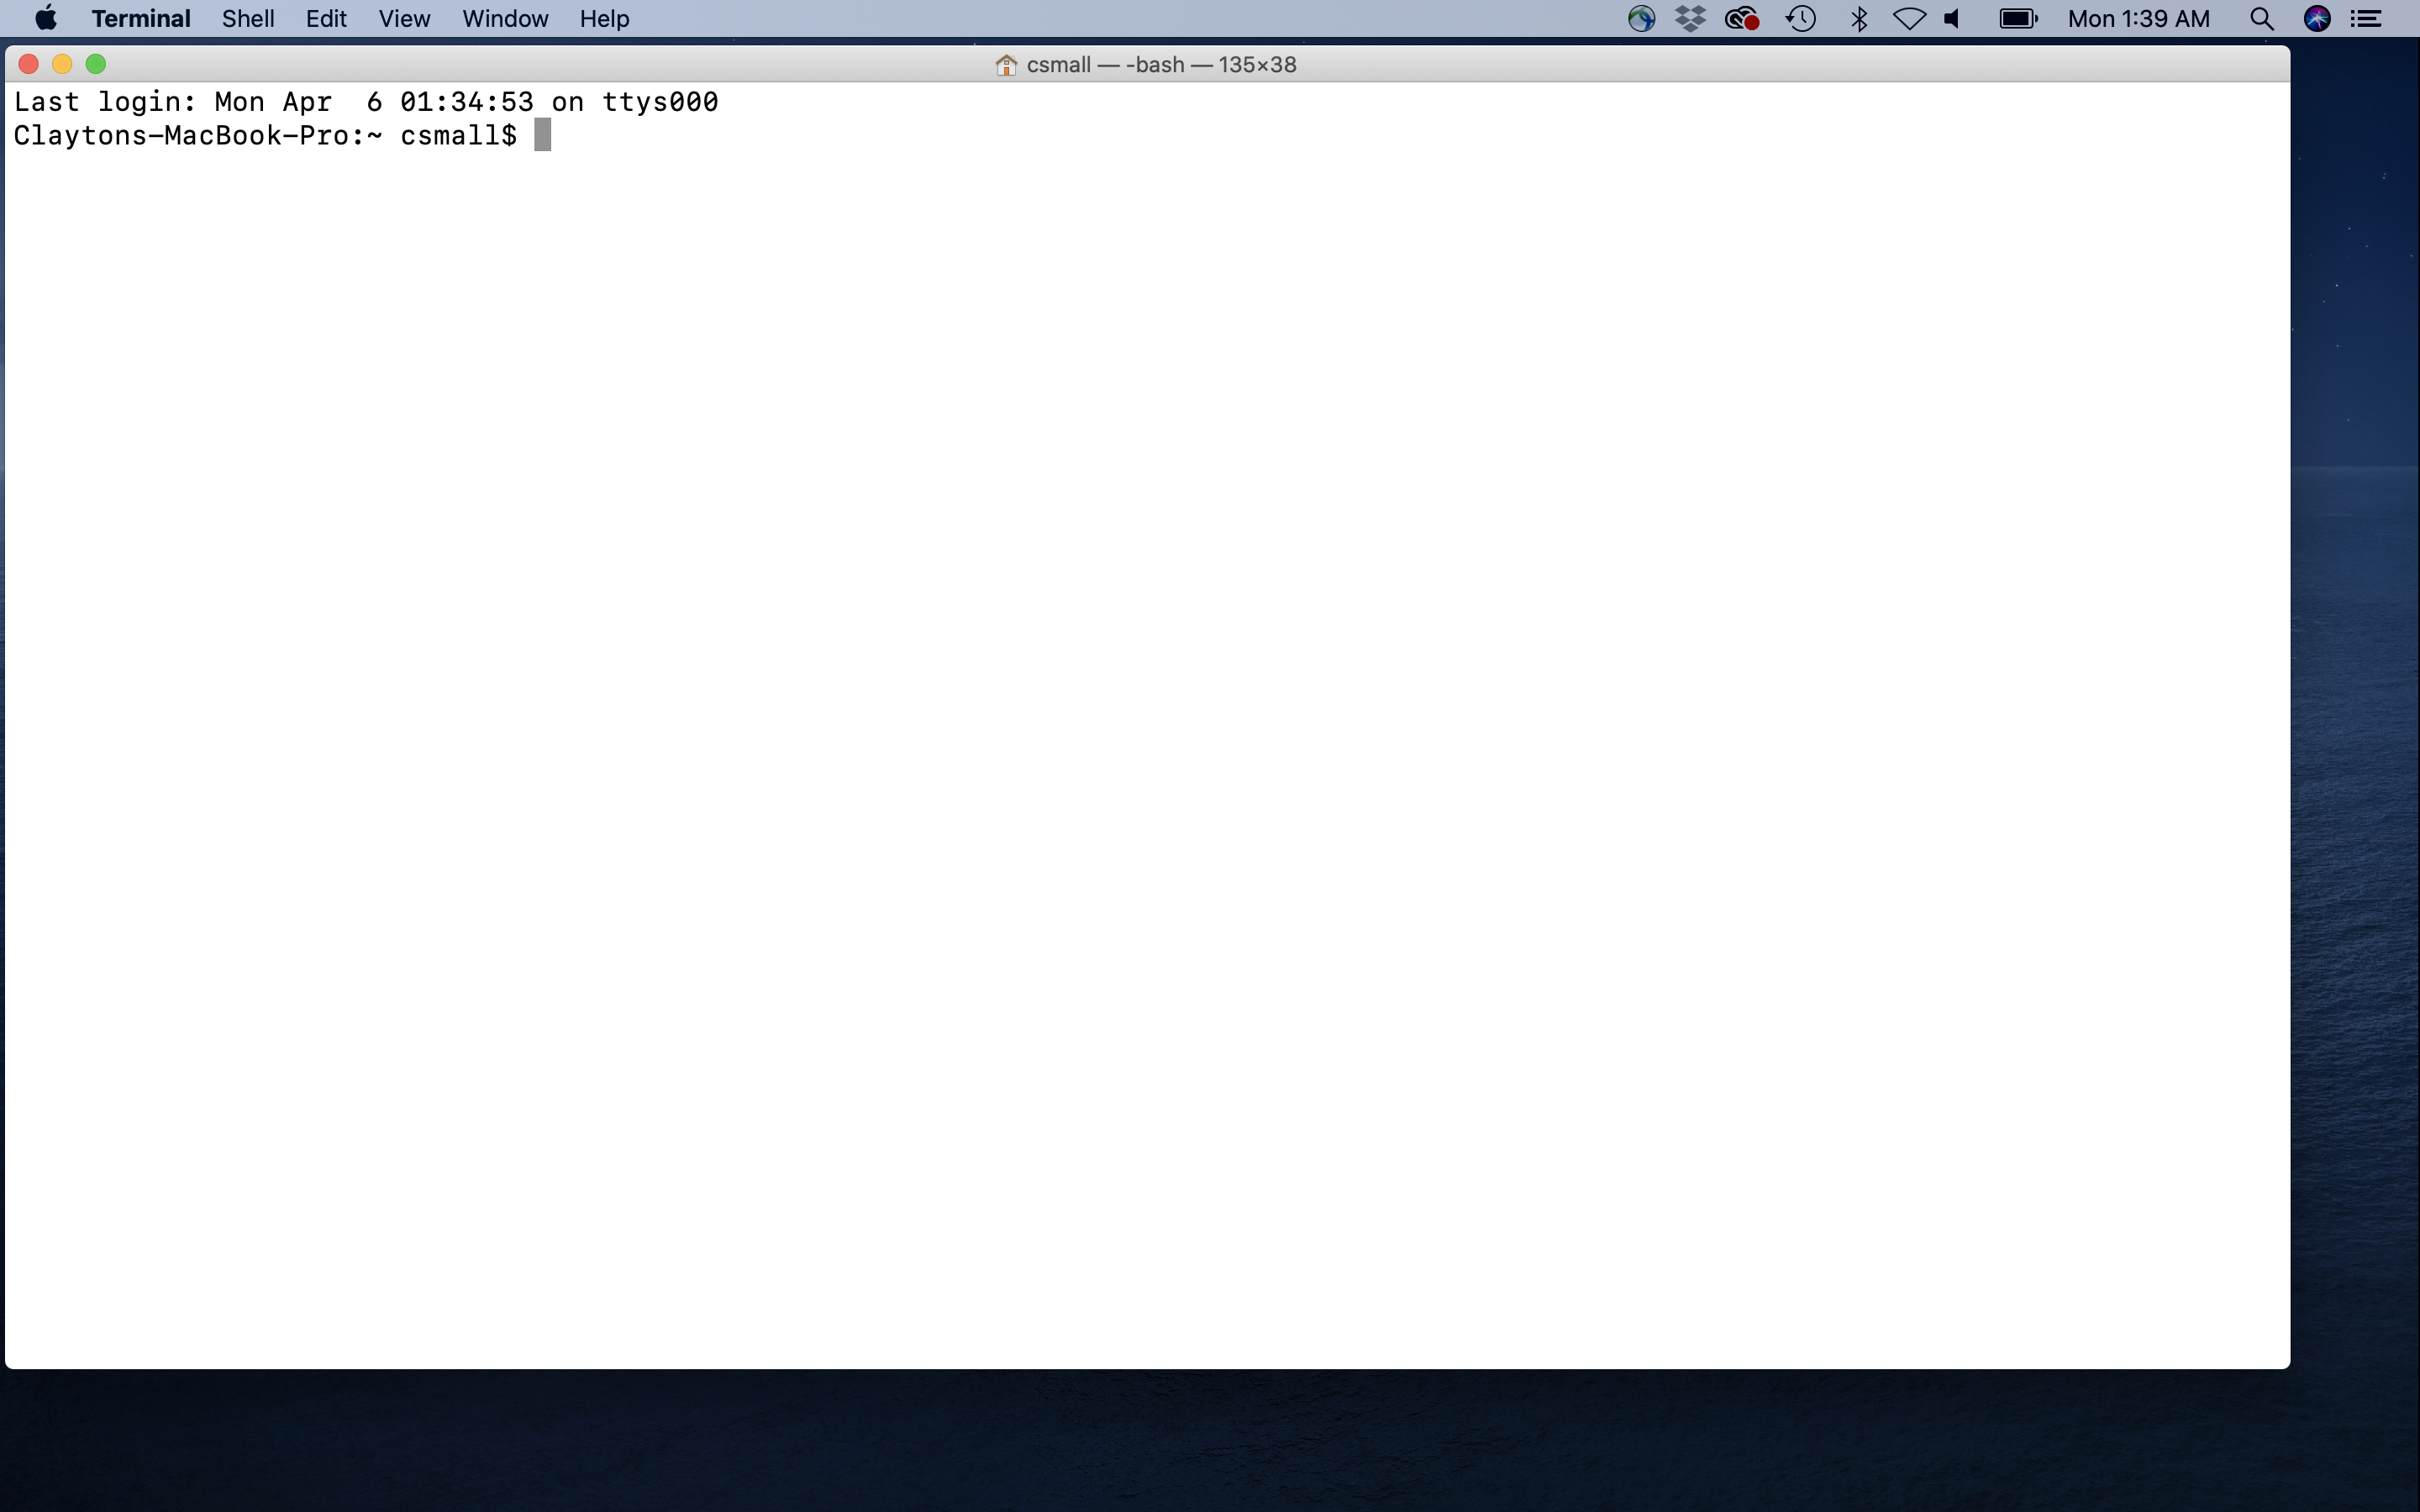
\includegraphics{/Users/csmall/github_repos/Found_Stat/images/MacTerminal.png}

You are now ready to navigate and explore files simply by typing!

\hypertarget{navigating-directories-and-files}{%
\subsection{Navigating directories and files}\label{navigating-directories-and-files}}

When you are at the command line, just think of your computer as you would if you were navigating using a graphical application (e.g.~Mac Finder or Windows Explorer). You are always in a directory in your file system, and you can move to any other directory by typing the approriate command and destination, then hitting Enter.

The first crucial UNIX command to learn is \texttt{pwd}. This command stands for ``print working directory,'' and it will literally print the path of the directory you are currently in.

Another important command is \texttt{ls}. This lists the files and directories (by default) in your working directory. If you specify a different directory, it will list the files and/or directories there. Most UNIX commands (and indeed command-line programs in general), can be run with options. One way to invoke the and option is to type a ``flag'' along with the command. In the case of \texttt{ls}, we can type \texttt{ls\ -l}, for example, which will print the output line-by-line. We can also add annother flag: \texttt{ls\ -lh} (equivalent to \texttt{ls\ -l\ -h}), which will print items line-by-line but also make sure the item sizes are ``human readable.'' If you ever have quesitons about how to use UNIX program, including the flags and other options, you can type \texttt{man\ program\_name} and a wonderful help manual will appear. To exit and return to the command prompt, just hit ``q''. These \texttt{man} pages are extremely useful and should be your first go-to if you need information for a particular command. Please use these regularly!

The command \texttt{cd} will change your location from the current directory to another directory. Like many other programs (UNIX and otherwise) require you to input directory and file locations, with \texttt{cd} you can specify your desired location using either the \emph{absolute} or \emph{relative} path. An absolute path is the full ``address'' of a directory or file, starting from the root of your file system. An example of an absolute path to a directory in my file system is \texttt{/Users/csmall/Dropbox/sculpin\_project/images/}. Regardless of where my current working directory is in my file system, I can change to this \texttt{images/} directory using \texttt{cd} and the full path. I can also use a relative path, which is a sort of ``shortcut,'' to specify the location of a directory or file. Let's say I am in \texttt{/Users/csmall/Dropbox/BiostatsFound\_S2020/} and I want to get to the \texttt{images/} directory above. I could type \texttt{cd\ ../sculpin\_project/images}, which uses a relative path to take me ``up'' one directory (as denoted by \texttt{../}) into \texttt{Dropbox/} and back ``down'' into \texttt{sculpin\_project/images}. In fact, \texttt{..} is a special file in every directory that just means ``the directory above.'' The special file \texttt{.} is the current directory. And to mention one final useful designation for navigation shortcuts, you can use the \texttt{\textasciitilde{}} to denote your home directory.

The schematic below should help you visualize how to think about file system navigation from the commmand line:
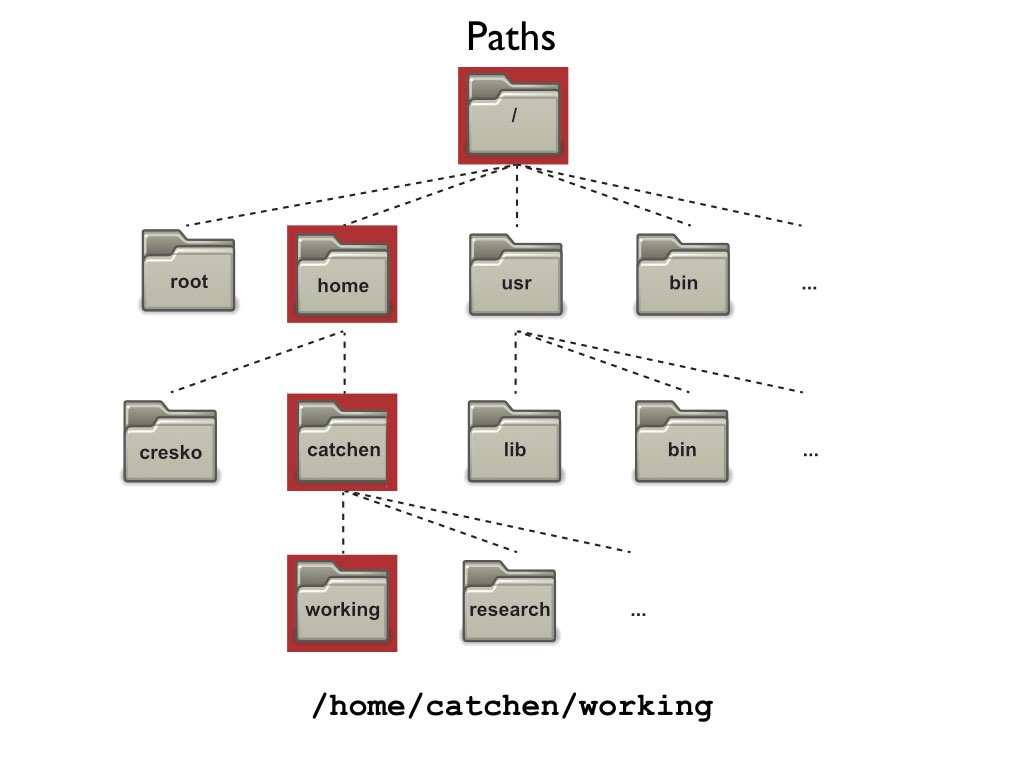
\includegraphics{/Users/csmall/github_repos/Found_Stat/images/Directory_example.jpeg}

And for another example, take a look at this series of navigation commands from my terminal and see if you can follow along:
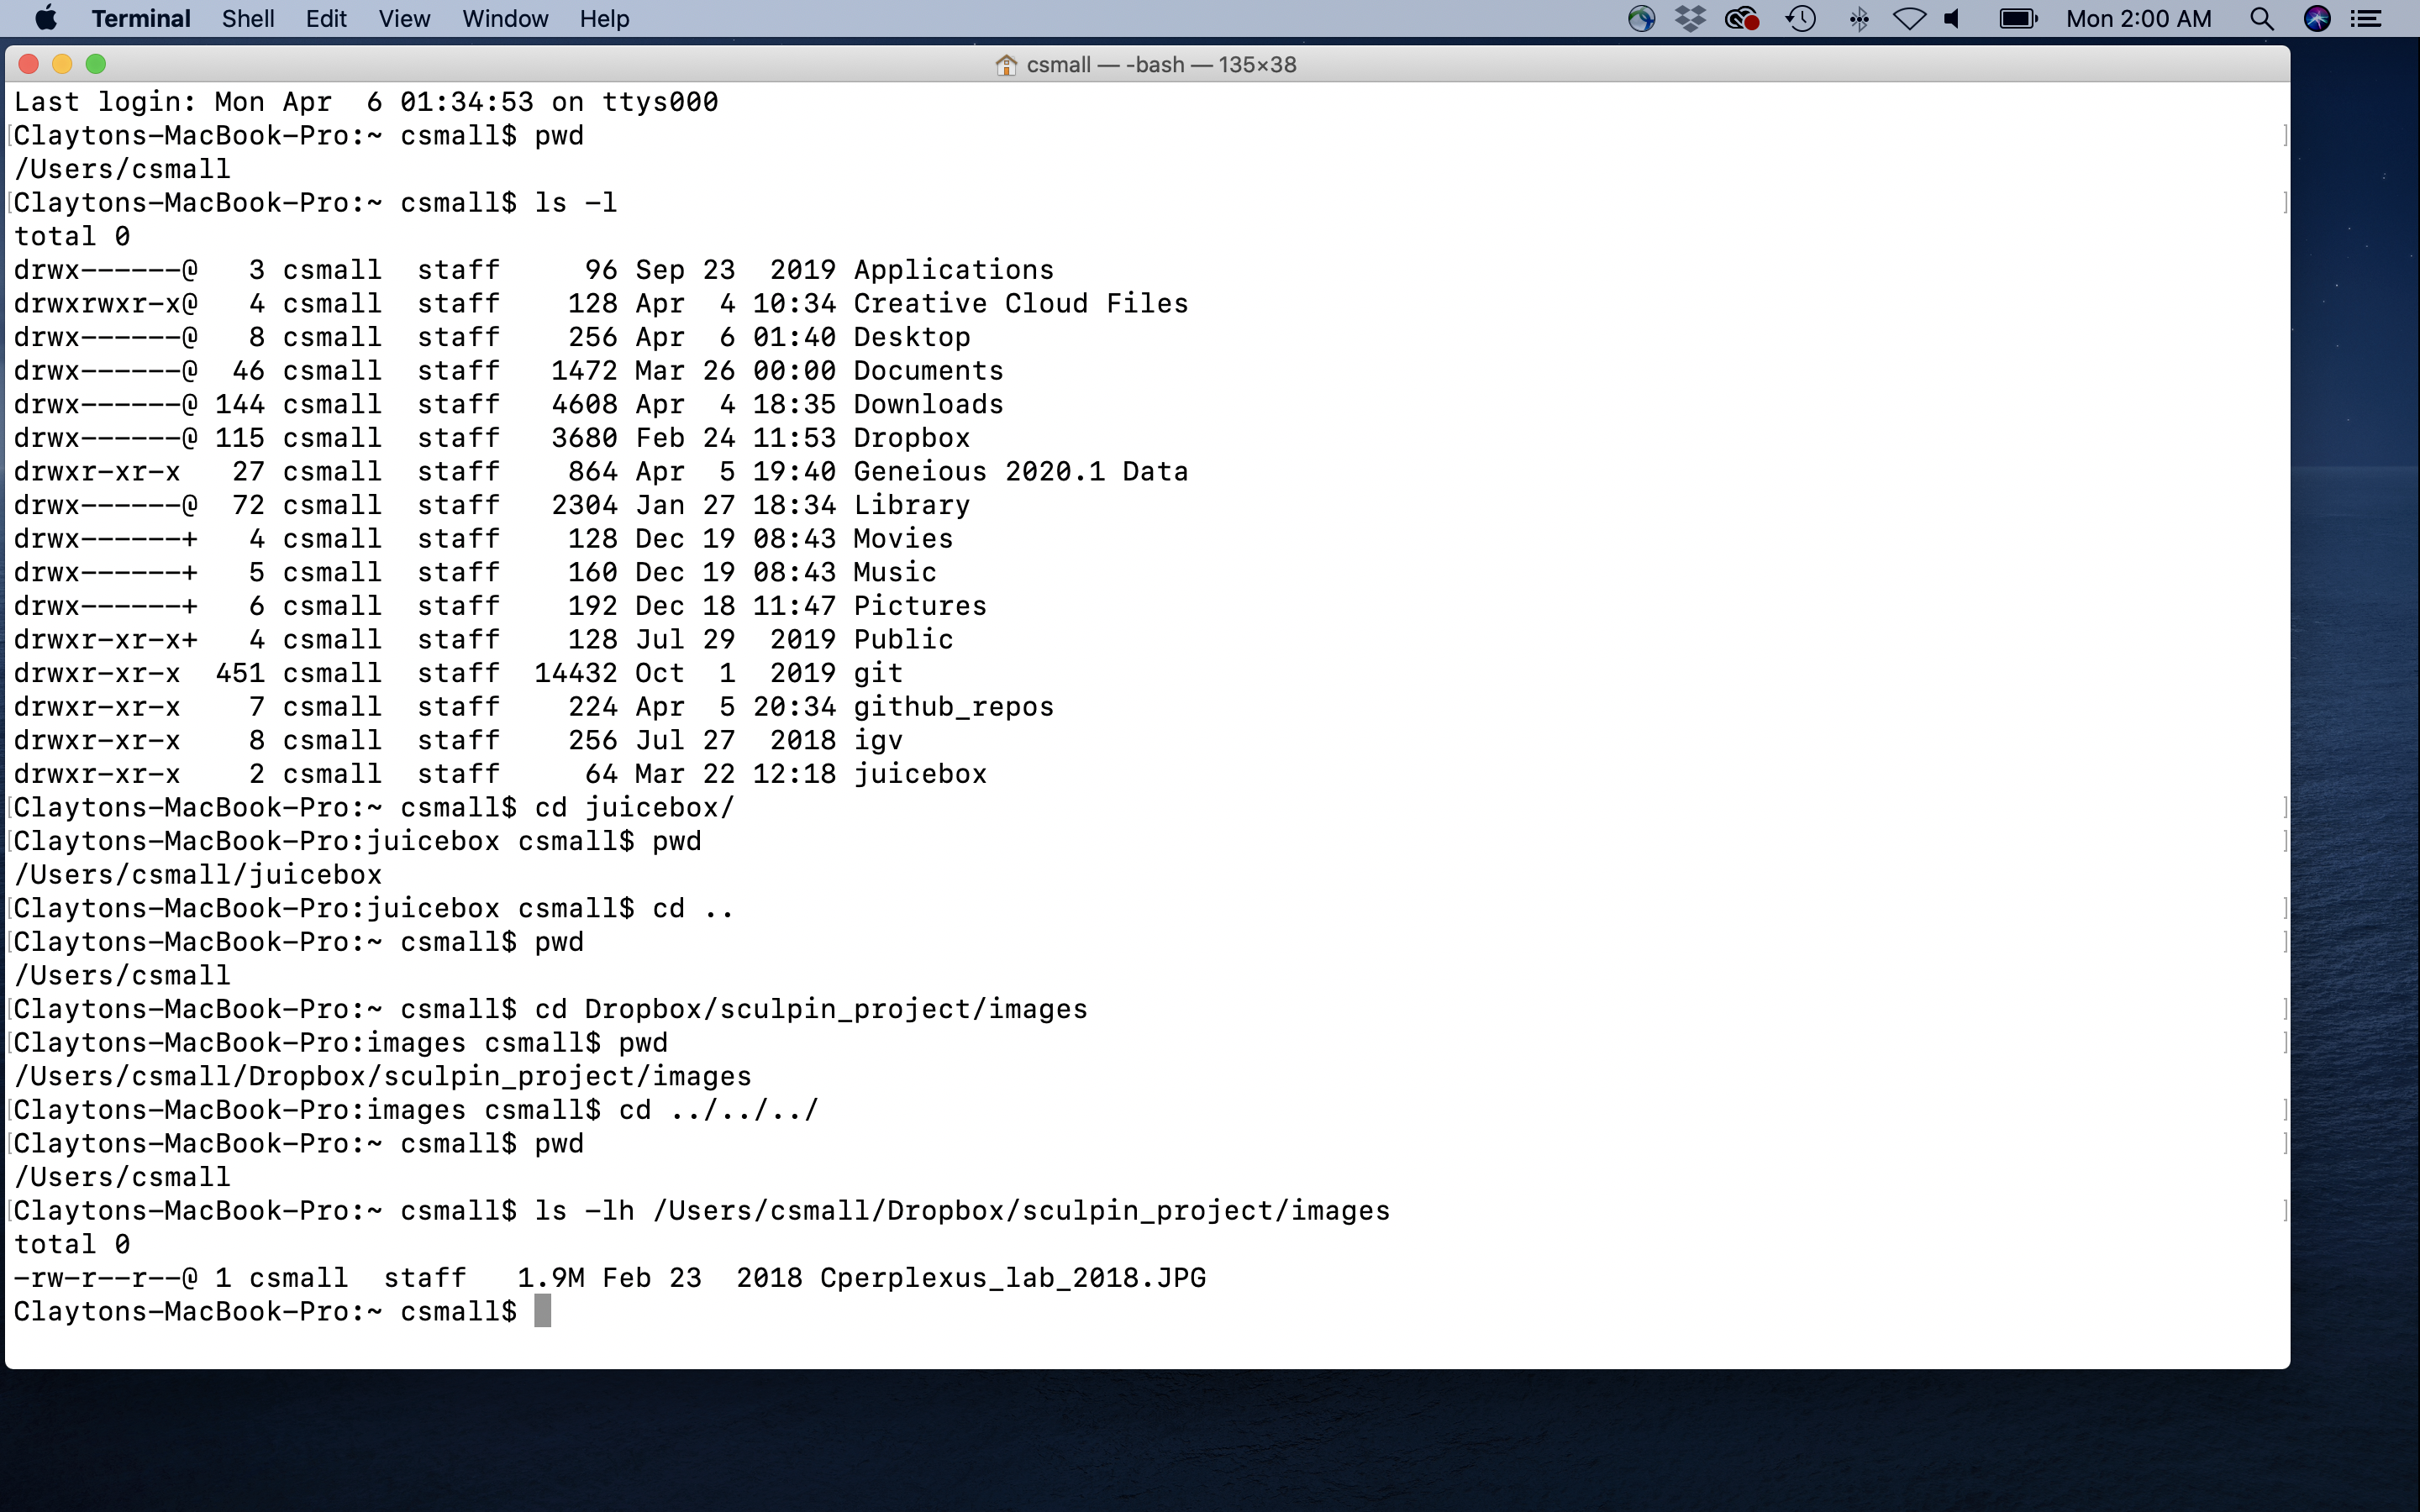
\includegraphics{/Users/csmall/github_repos/Found_Stat/images/MacTerminal_2.png}

If you want to create a new directory, you can use the \texttt{mkdir} command, including the desired name of the new directory. By default this will create the directory in your current working directory, but you can use absolute or relative paths to instead write the directory somewhere else. If you want to delete an empty directory, \texttt{rmdir} is the appropriate command.

Now let's briefly cover some UNIX commands that are useful for managing files. Some of these apply to directories as well, which I will point out as we go. The command \texttt{touch} can be used to create a new, empty file, which you can add to using a plain text editor. Examples of popular plain text editors with advanced user interfaces are BBEdit and Atom. You can also use command line text editors, such as \texttt{nano}, \texttt{emacs}, and \texttt{vim}. Most UNIX/LINUX systems have \texttt{nano} installed by default. To copy or change the name and/or location of a file (or directory), use \texttt{cp} and \texttt{mv} commands, respectively. Note that by using absolute or relative paths, you can specify where you want the file or directory to end up. Be especially careful with these, however, because you will overwrite any existing file or directory if you specify the same name and location. Another command you should be extremely cautious with is \texttt{rm}, which removes (permanently deletes) a file. \texttt{rm\ -r} can be used to delete a non-empty directory AND all of its contents.

In many cases you will want to look at files, or parts of them at least, from the command line. \texttt{cat} will print the entire contents of a file, but can also be used to combine (``concatenate'') multiple files in a line-wise manner. \texttt{less} and \texttt{more} will display specific lines of a file (starting with the first ones), with single- or multi-line ``scrolling,'' respectively, activated using the return or down-arrow keys. To leave the display, you need to hit the ``q'' key. \texttt{head} and \texttt{tail} will display the first or last, respectively, \emph{n} lines of the file, where \emph{n} is provided as a flag (e.g. \texttt{head\ -200\ file.tsv}). The ``word count'' command \texttt{wc} can quantify elements of a text file in various ways, but one common application is \texttt{wc\ -l}, which counts the number of lines in a file.

An aside: If you are working from the command line and want to terminate a process (say you accidentally start a task that will take way too long), press Ctrl-C.

\hypertarget{a-quick-review-of-important-unix-commands-for-navigation-and-viewing}{%
\subsubsection{A quick review of important UNIX commands for navigation and viewing}\label{a-quick-review-of-important-unix-commands-for-navigation-and-viewing}}

\texttt{pwd} - prints working directory

\texttt{ls} - lists contents of a directory

\texttt{cd} - changes the working directory

\texttt{mkdir} - creates a new directory

\texttt{rmdir} - deletes an empty directory

\texttt{touch} - creates an empty file

\texttt{cp} - copies a file or directory

\texttt{mv} - changes the name of a file or directory

\texttt{rm} - deletes a file, or a directory and everyting inside with \texttt{-r}

\texttt{cat} - prints the entire file to the terminal, or concatenates and prints multiple files

\texttt{less} - displays the first lines of a file, with scrolling line-by-line

\texttt{head} - prints the first 10 lines (default) of a file

\texttt{tail} - prints the last 10 lines (default) of a file

\texttt{wc\ -l} - prints the number of lines in a file

\hypertarget{useful-unix-commands-for-file-manipulation}{%
\subsection{Useful UNIX commands for file manipulation}\label{useful-unix-commands-for-file-manipulation}}

In many cases you will want to search for specific characters or combinations of characters, and do various things with that information. Maybe you want to isolate the lines of a file that contain the query, or perhaps you want to count how many lines contain the query. The tool \texttt{grep} is extremely useful in this regard. We don't have time for a comprehensive dive into the utilities of \texttt{grep}, but a few common applications are worth mentioning. Character patterns we search for using \texttt{grep} may or may not involve special characters that are not interpretted literally. Here we will discuss just a few common cases of \texttt{grep} searches and the special characters involved. Some examples of these special characters include \texttt{\^{}} (beginning of a line), \texttt{\$} (end of a line), \texttt{.} (any single character except a newline), \texttt{*} (zero or more instances of the preceeding character), and \texttt{\textbackslash{}s} (any white space). The standard syntax for \texttt{grep} from the command line is \texttt{grep\ "expression"\ filename}. So, if you wanted to return all of the lines in the data file \texttt{zfish\_data.tsv} (assuming it is in the current directory) that begin with ``embryo\_10'', you could try \texttt{grep\ "\^{}embryo\_10"\ zfish\_data.tsv}. This search would also (unintentionally) find lines beginning with ``embryo\_100'' or ``embryo\_101'', etc., if they exist. So, you have to be careful, and learning the rules just takes practice. In this case \texttt{grep\ "\^{}embryo\_10\textbackslash{}s"\ zfish\_data.tsv} would acheive the desired result, assuming that there is a whitespace delimiter between fields (``columns'') in the data file. Useful flags for \texttt{grep} include \texttt{-c} (which counts the number of lines containing the query), \texttt{-v} (which returns the lines that \emph{do not} contain the query), and \texttt{-n} (which prints the line number for each line containing the query). I encourage you to look at many different \texttt{grep} use cases online as your demand for complex searches grows.

The program \texttt{sed} has reasonably complex applciations, but is commonly used as a sort of ``search and replace'' tool. The syntax for \texttt{sed} use is similar to \texttt{grep}, except that the query and replacement expressions are organized (with other information) using slashes. For ``search and replace'' functionality, that sytax looks like this: \texttt{sed\ \textquotesingle{}s/query/replacement/flag\textquotesingle{}\ filename}. One common option for the ``flag'' component is ``g'', meaning ``global'', which replaces all instances. If no flag designation is made only the first instance in the file is replaced. Building on our toy example from above, \texttt{sed\ \textquotesingle{}s/\^{}embryo\_/\^{}larva\_/g\textquotesingle{}\ zfish\_data.tsv} would perform a global replacement and print the output to the terminal. To change the contents in the original file on the fly, including \texttt{sed\ -i} would do the trick, but is riskier than redirecting the output to a new file.

\texttt{cut} is quite straightforward, and can be used to isolate individual fields (think of them like ``columns'') from a text file, provided the fields are consistently separated by a delimeter on each line. So, if I had a comma-separated file and I just wanted the first two columns I could type \texttt{cut\ -f1,2\ -d"\textbackslash{}t"\ filename}. Note that if you don't specify a delimter using the \texttt{-d} flag, then it is assumed to be tab-delimited. If you want to bring together fields in separate files, \texttt{join} can be used to accomplish this. The two files should have equivalent rows, however, for this action to work properly.

If you want to sort text files alphanumerically, in a field-wise fashion, \texttt{sort} is quite useful. If a file contains a single field, minimal specification is required, aside from tuning numerical sorting. For example, if you want to sort numerically, use the \texttt{-n} flag, and if you want to sort from largest to smallest, add the \texttt{-r} flag. If you want to sort a multi-field file based on just one field, you can use the ``key'' flag. For instance, if you have a tab-delimited file and want to sort by the second field in reverse numerical order, \texttt{sort\ -k2,2\ -nr\ filename.tsv} would give you the desired result. Finally, if you want to eliminate lines with the same value for a given field, you can use the \texttt{-u} ``unique'' flag.

The UNIX program \texttt{awk} is an extremely powerful tool, and can itself be used essentially as a mini programming language. We will not get into the myriad uses of \texttt{awk} here, but the reference at the bottom of the chapter is a great resource if you want to learn more. \texttt{awk} is extremely efficient at parsing and capturing text files in a column-wise manner, with the ability to also evaluate logical statements applied to rows. The structure of \texttt{awk} commands is more complex than that of other UNIX programs we have discussed, but it is still very intuitive. One unique feature is that \texttt{awk} contains its own internal functions, which are typed inside curly braces. The ``print'' function can be used to extract fields, much like \texttt{cut}. For instance, \texttt{awk\ -F:\ \textquotesingle{}\{print\ \$1,\$6\}\textquotesingle{}\ filename.tsv} would print the first and sixth field from \texttt{filename.tsv}, assuming a ``:'' delimiter. With \texttt{awk}, fields are specified using the \texttt{\$} character. If you want also to select only specific rows from a set of columns (like those with a certain value), you can incorporate logical operators. In the above example if we had wanted fields 1 and 6, but only those rows with a value of at least 610 in field 2, we could type the following \texttt{awk\ -F:\ \textquotesingle{}\$4\ \textgreater{}=\ 610\ \{print\ \$1,\$6\}\textquotesingle{}\ filename.tsv}. Again, this is just scratching the surface with \texttt{awk}, which boasts a great deal of potential for your text file manipulation needs.

\hypertarget{a-quick-review-of-key-unix-commands-for-text-file-searching-and-manipulation}{%
\subsubsection{A quick review of key UNIX commands for text file searching and manipulation}\label{a-quick-review-of-key-unix-commands-for-text-file-searching-and-manipulation}}

\texttt{grep} - searches a file for characters and character combinations

\texttt{sed} - stream edits characters and character combinations

\texttt{cut} - isolates specific fields (``columns'') from a file using a delimiter

\texttt{join} - combines fields (``columns'') from multiple files with equivalent rows

\texttt{sort} - orders the rows in a file based on one or more fields

\texttt{awk} - flexibly parses, evaluates, and selectively prints row- and column-wise

\hypertarget{a-quick-word-on-pipes-and-carrots}{%
\subsection{A quick word on pipes and carrots}\label{a-quick-word-on-pipes-and-carrots}}

One very convenient feature of UNIX commands is that you can control the flow of input and output from one command to another using the \texttt{\textbar{}} (``pipe'') character. For instance, I may want to search an entire file for rows that begin with ``fish-1'', and then replace the ``-'' with "\_``. To do this I could do something like \texttt{cat\ file.tsv\ \textbar{}\ grep\ "\^{}fish-1"\ \textbar{}\ sed\ \textquotesingle{}s/fish-1/fish\_1/g\textquotesingle{}} This, of course, would print the output to the terminal, but I could actually capture that output into a file using the \texttt{\textgreater{}} charcter. \texttt{cat\ filename\ \textbar{}\ grep\ "\^{}fish-1"\ \textbar{}\ sed\ \textquotesingle{}s/fish-1/fish\_1/g\textquotesingle{}\ \textgreater{}\ ./newfile.tsv} would write this new file to my current working directory. Furthermore, if you want to append lines of text to an existing file, the''double sideways right-pointing carrot" character \texttt{\textgreater{}\textgreater{}} can be used.

The above lessons on UNIX commands for file manipulation truly just scratch the surface of what can be accomplished at the command line and in ``shell scripts.'' You certainly will have further questions and be hungry for more, but we simply don't have time during this course. But to work on your UNIX skills for now, check out \texttt{Ex1\_Unix\_Intro.html} (on Canvas). We need to move on to R now, but at the bottom of this chapter are some UNIX command resources I have found to be especially useful.

\hypertarget{data-file-and-data-file-entry-dos-and-donts}{%
\section{Data file and data file entry dos and don'ts}\label{data-file-and-data-file-entry-dos-and-donts}}

Do store a copy of your data in a nonproprietary format, such as plain ASCII text (aka a flat file). This is especially important if you are using tools (like UNIX commands) to parse and manipulate the files. Formats like Microsoft Excel are not acceptable as input for many analysis tools, and not everyone has access to proprietary software.

Do leave an un-edited copy of an original data file, even when main analyes require an edited version.

Do use descriptive names for your data files and variables, and use them consistently!

Do maintain effective metadata about the data.

Do add new observations to a data file as rows.

Do add new variables to a data file as columns.

Don't include multiple data types in the same column.

Don't use non-alphanumeric characters (other than the underscore) in file or directory names.

Don't use spaces, tabs, commas, colons, semicolons, or other chacters commonly used as field (column) delimiters in names of individual data entries. For example, don't use something like \texttt{March\ 8} as a value for date in a data set.

Don't copy and paste data directly from rich-text-formatted files (like Microsoft Word) into primary data files.

\hypertarget{exercises-associated-with-this-chapter}{%
\section{Exercises associated with this chapter:}\label{exercises-associated-with-this-chapter}}

\begin{itemize}
\tightlist
\item
  Exercise 1 (file: \texttt{Ex1\_Unix\_Intro.html})
\end{itemize}

\hypertarget{additional-learning-resources}{%
\section{Additional learning resources}\label{additional-learning-resources}}

\begin{itemize}
\item
  \url{http://mally.stanford.edu/~sr/computing/basic-unix.html} - A nice ``cheat sheet''
\item
  \url{http://korflab.ucdavis.edu/Unix_and_Perl/} - Outstanding tutorial by Keith Bradnam and Ian Korf
\item
  \url{https://www.datacamp.com/courses/introduction-to-shell-for-data-science} - DataCamp tutorial
\item
  \url{https://www.gnu.org/software/gawk/manual/gawk.html} - A comprehensive guide to \texttt{awk}
\end{itemize}

\hypertarget{an-introduction-to-the-r-language}{%
\chapter{An Introduction to the R language}\label{an-introduction-to-the-r-language}}

\hypertarget{background}{%
\section{Background}\label{background}}

\texttt{R} is a computer programming language and environment especially useful for graphic visualization and statistical analysis of data. It is an offshoot of a language developed in 1976 at Bell Laboratories called \texttt{S}. \texttt{R} is an interpreted language, meaning that every time code is run it must be translated to machine language by the \texttt{R} interpreter, as opposed to being compiled prior to running. \texttt{R} is the premier computational platform for statistical analysis thanks to its GNU open-source status and countless packages contributed by diverse members of the scientific community.

\hypertarget{why-use-r}{%
\section{\texorpdfstring{Why use \texttt{R}?}{Why use R?}}\label{why-use-r}}

\begin{itemize}
\tightlist
\item
  Good general scripting tool for statistics and mathematics
\item
  Powerful and flexible and free
\item
  Runs on all computer platforms
\item
  New packages released all the time
\item
  Superb data management \& graphics capabilities
\item
  Reproducibility - can keep your scripts to see exactly what was done
\item
  Can embed your \texttt{R} analyses in dynamic, polished files using R markdown
\item
  You can write your own functions
\item
  Lots of online help available
\item
  Can use a nice IDE such as \texttt{RStudio}
\end{itemize}

\hypertarget{important-r-terms-and-definitions}{%
\section{\texorpdfstring{Important \texttt{R} terms and definitions}{Important R terms and definitions}}\label{important-r-terms-and-definitions}}

\begin{figure}
\centering
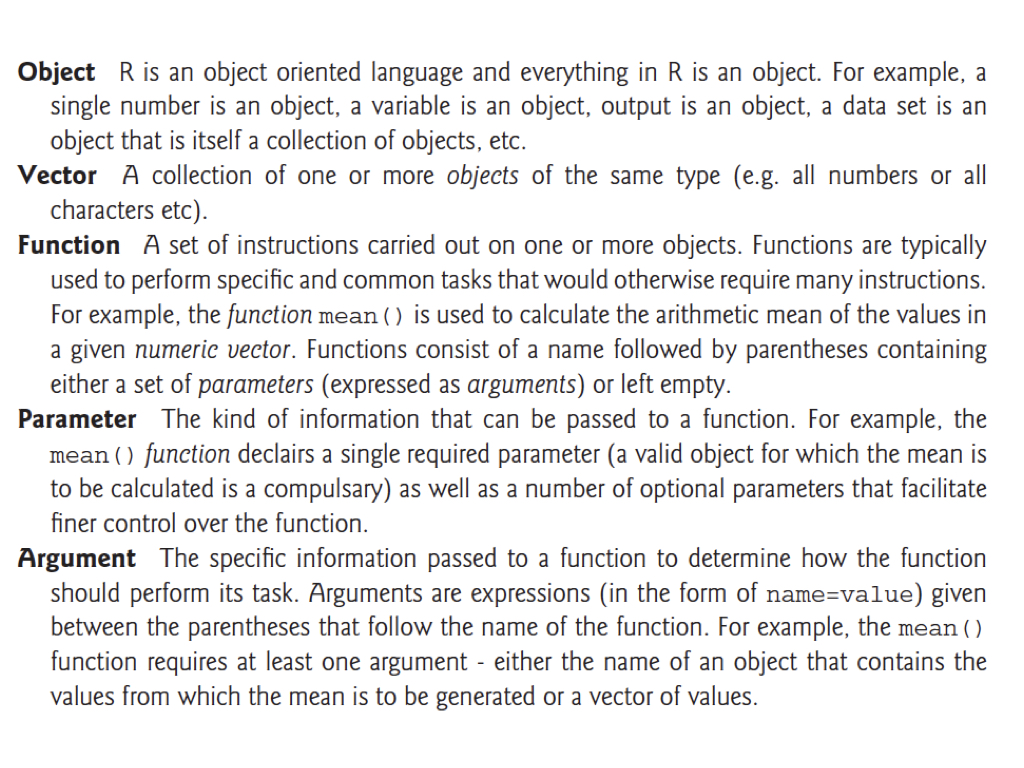
\includegraphics{/Users/csmall/github_repos/Found_Stat/images/R_definitions_Logan.001.jpeg}
\caption{Alt text}
\end{figure}

From Logan, M. 2010. \emph{Biostatistical Design and Analysis Using R}

Operators are symbols in programming that have a specific meaning

\begin{figure}
\centering
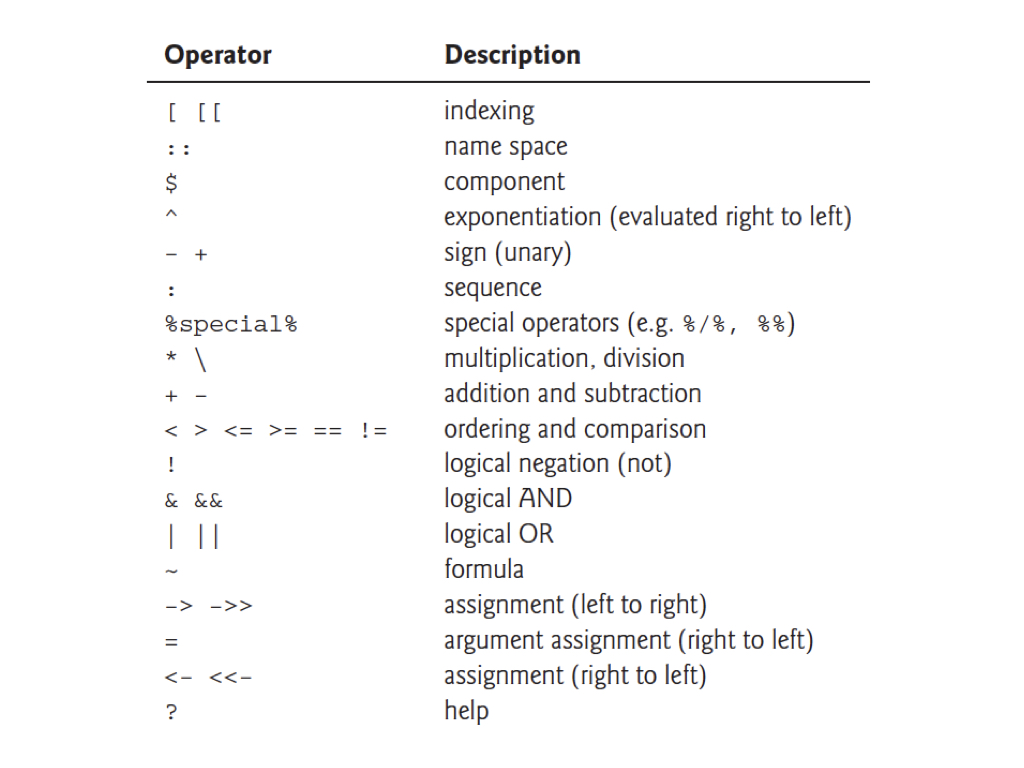
\includegraphics{/Users/csmall/github_repos/Found_Stat/images/R_definitions_Logan.002.jpeg}
\caption{Alt text}
\end{figure}

From Logan, M. 2010. \emph{Biostatistical Design and Analysis Using R}

\hypertarget{getting-started-with-r-via-the-rstudio-environment}{%
\section{\texorpdfstring{Getting started with \texttt{R} via the RStudio Environment}{Getting started with R via the RStudio Environment}}\label{getting-started-with-r-via-the-rstudio-environment}}

To begin working with \texttt{R}, open RStudio. You should first see something that looks like this:
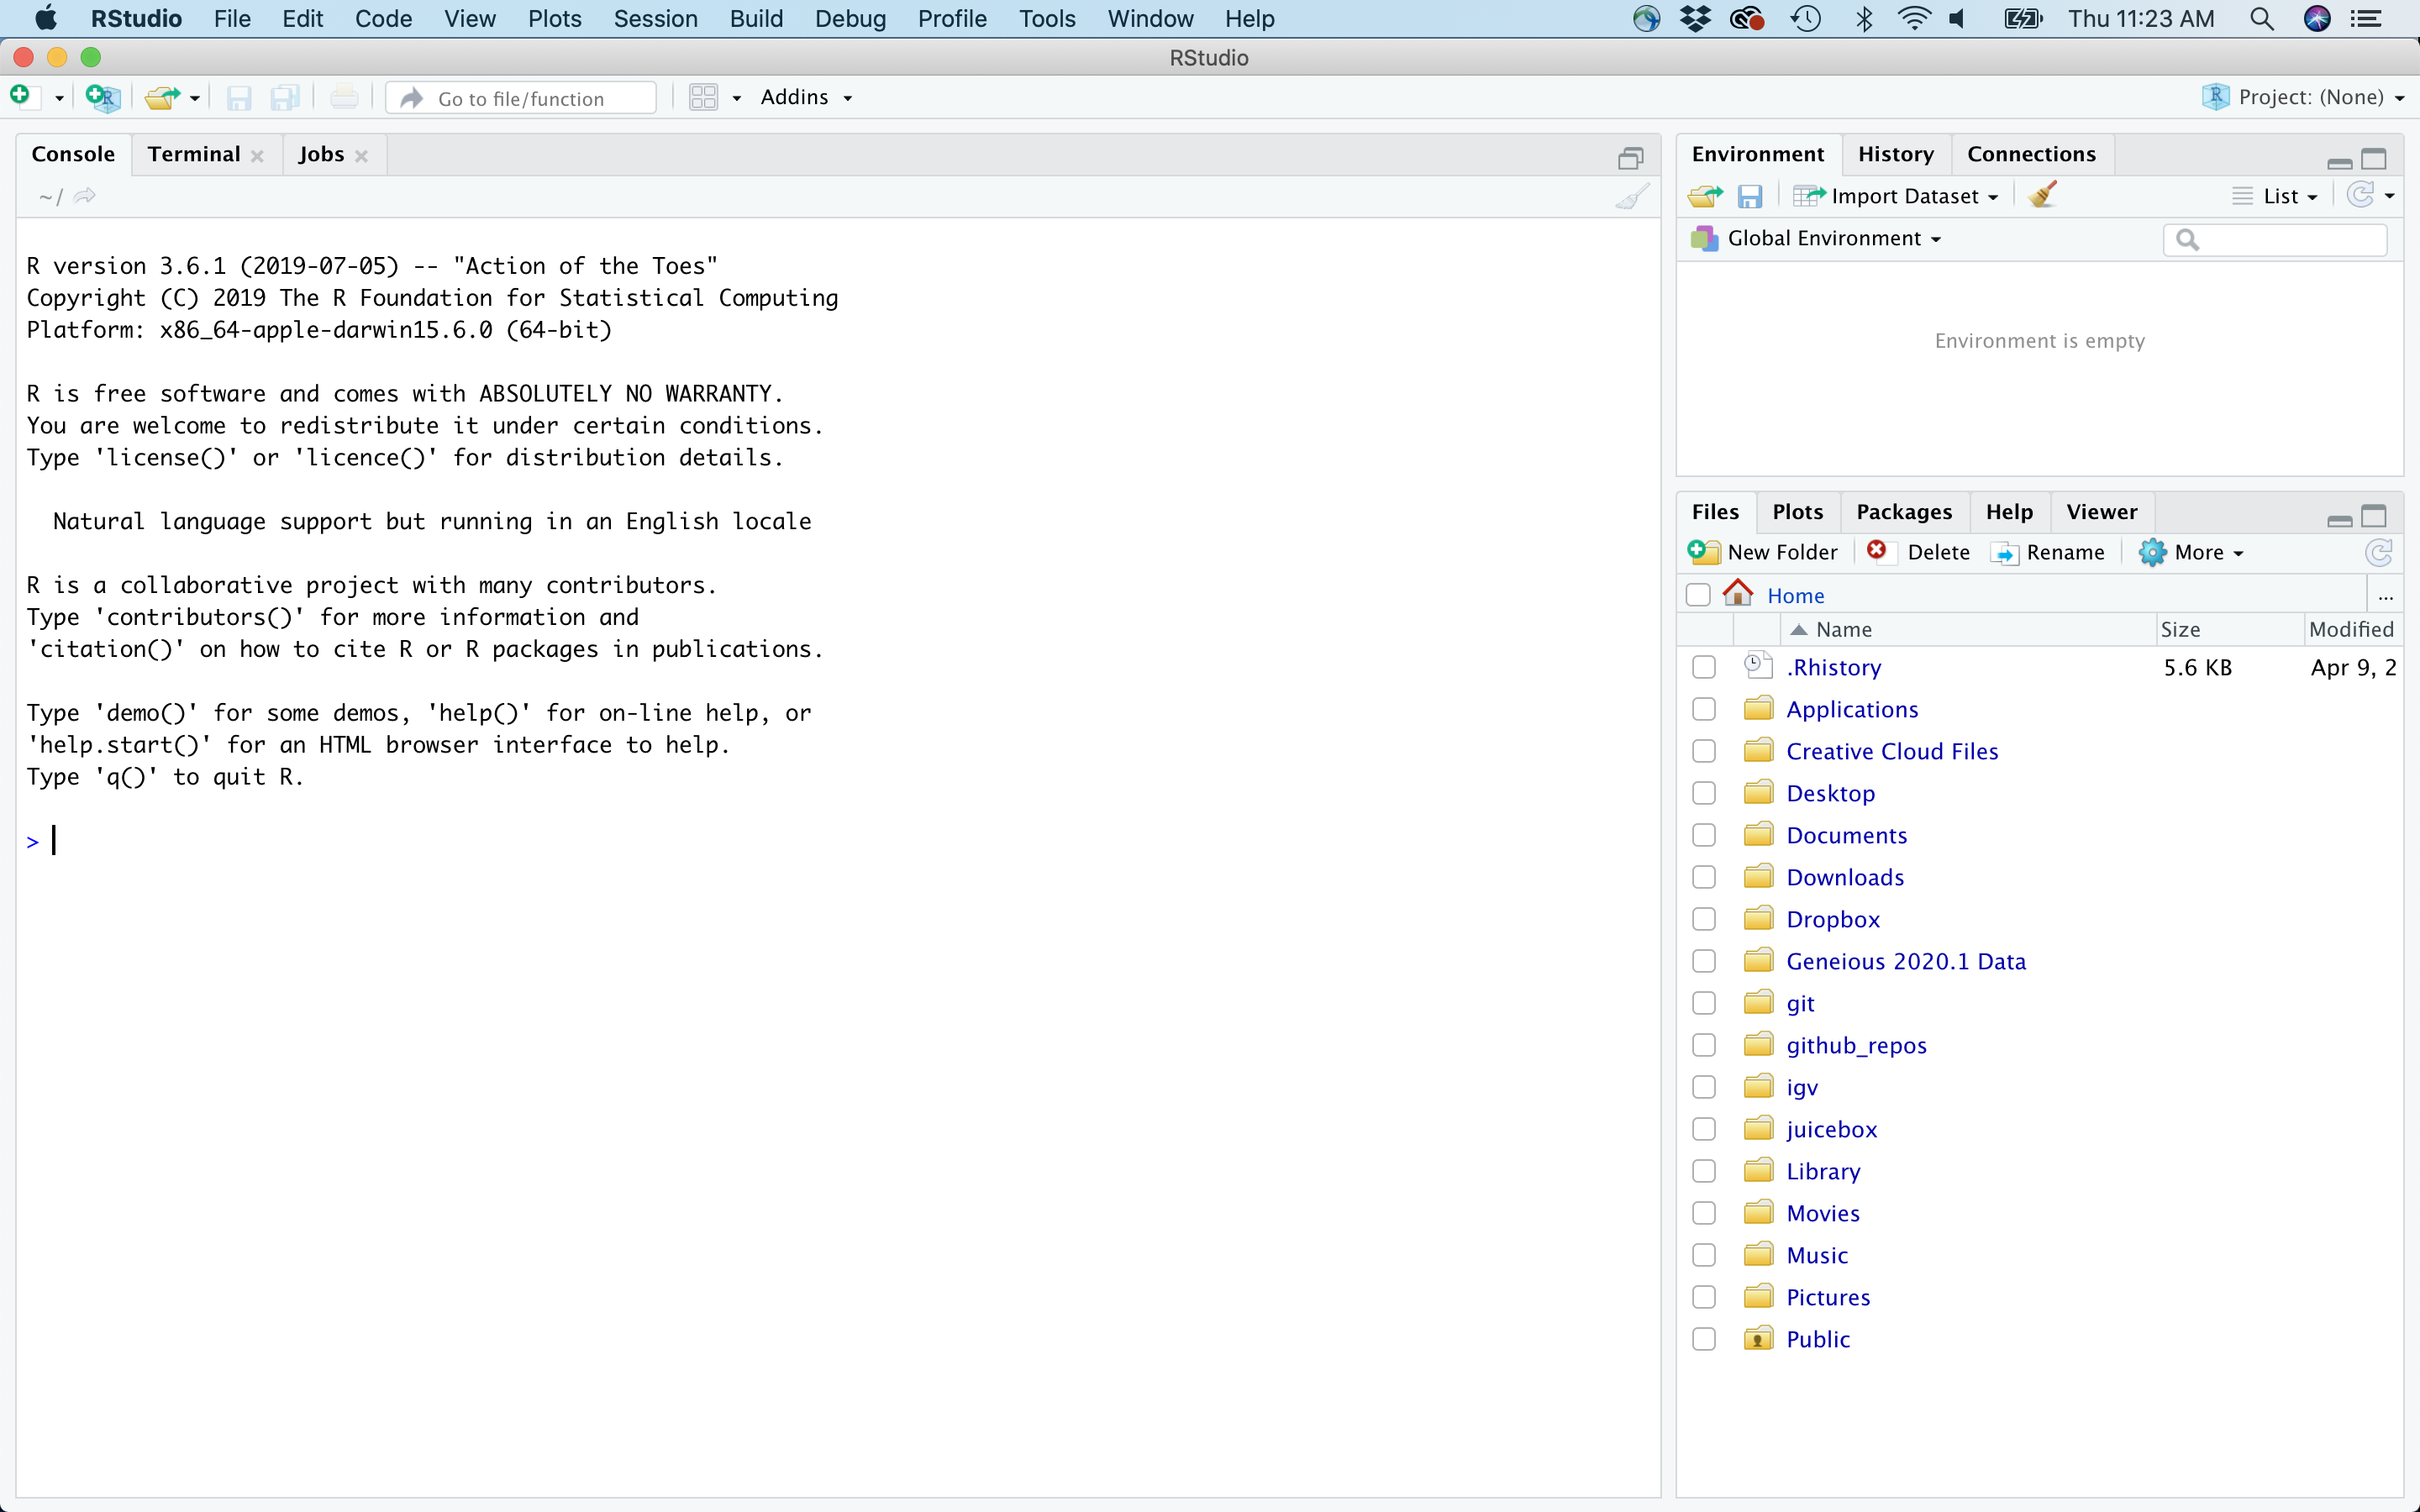
\includegraphics{/Users/csmall/github_repos/Found_Stat/images/MacTerminal_3.png}

To open a new script editor (where you will keep track of your code and notes), go to File \textgreater{} New File \textgreater{} R Script. Note that there are other options for file types, which we will be using in the future. For now, though, we want a plain script, which when saved will have the extention \texttt{.R}.

It is easy to run code directly from the script editor. For single lines of code, simply make sure your cursor is on that line, and hit Ctrl-Enter. For multiple lines, highlight the block of code you want to run and hit Ctrl-Enter.

Now your display should look somehting like below (but without the red pane labels, of course):
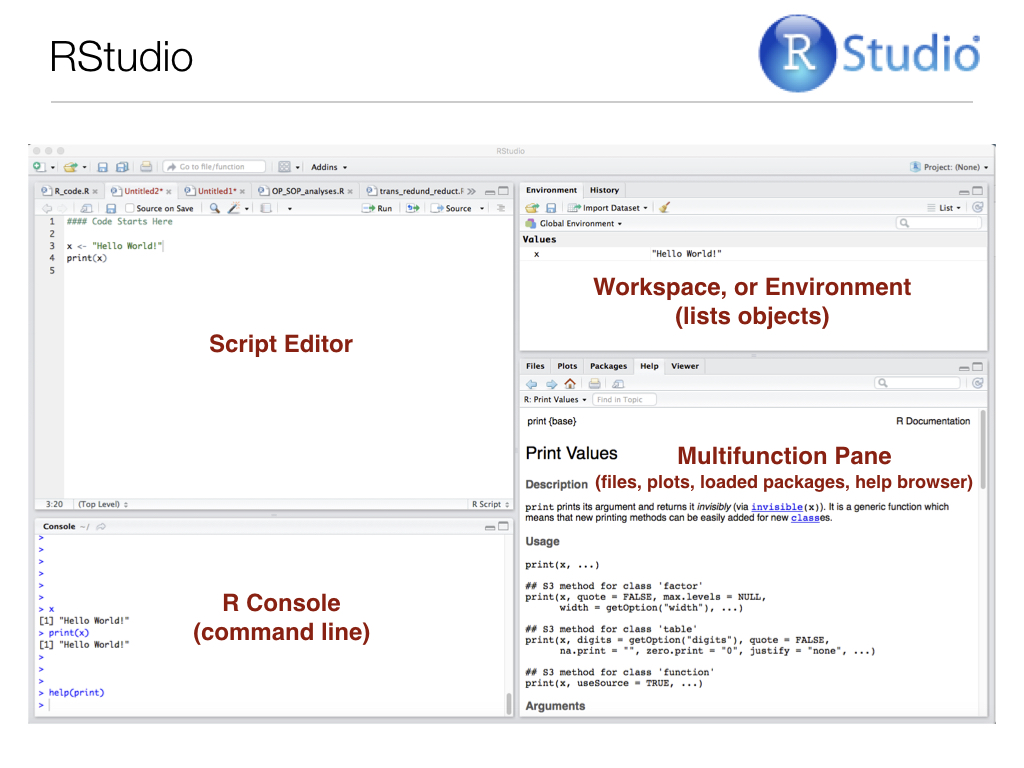
\includegraphics{/Users/csmall/github_repos/Found_Stat/images/R_definitions_Logan.003.jpeg}

Note that you can also type commands directly from the command line using the \texttt{R} Console (lower left pane), and the \texttt{R} interpreter will run them when you press Enter.

Any objects you define, and a summary of their values, will appear in the upper right pane, and the lower right pane differs in appearance depending on instructions you provide to \texttt{R\ Studio}. For instance, if you produce a plot, it will appear there by default. Another extremely important feature of R functions (we'll get to them in a bit) is the help file. Recall from Chapter 5 our discussion of \texttt{man} pages for UNIX programs. Help files the equivalent for \texttt{R} functions. They contain almost everything you need to know about a given function, and most of them even include and example at the bottom. These help files will appear in the lower right RStudio pane when you call them, for example when you run \texttt{help(function\_name)} at the \texttt{R} Console.

\hypertarget{r-programming-basics}{%
\subsection{R Programming Basics}\label{r-programming-basics}}

For the code examples below, it might be useful for you to start your own RStudio session, open a new \texttt{.R} file and type/run code while reading.

\begin{itemize}
\tightlist
\item
  Commands can be submitted through the terminal, console or scripts
\item
  In your scripts, anything that follows \texttt{\#} symbol (aka hash) is just for humans
\item
  Notice on these slides I'm evaluating the code chunks and showing output
\item
  The output is shown here after the two \texttt{\#} symbols and the number of output items is in \texttt{{[}{]}}
\item
  Also notice that \texttt{R} follows the normal priority of mathematical evaluation
\end{itemize}

\begin{Shaded}
\begin{Highlighting}[]
\DecValTok{4}\OperatorTok{*}\DecValTok{4}
\end{Highlighting}
\end{Shaded}

\begin{verbatim}
## [1] 16
\end{verbatim}

\begin{Shaded}
\begin{Highlighting}[]
\NormalTok{(}\DecValTok{4}\OperatorTok{+}\DecValTok{3}\OperatorTok{*}\DecValTok{2}\OperatorTok{^}\DecValTok{2}\NormalTok{)}
\end{Highlighting}
\end{Shaded}

\begin{verbatim}
## [1] 16
\end{verbatim}

\hypertarget{a-note-on-r-markdown}{%
\subsubsection{\texorpdfstring{A note on \texttt{R} Markdown}{A note on R Markdown}}\label{a-note-on-r-markdown}}

This format provides a much better way to embed code and output, in an easily readable, reproducible manner. We will dive into \texttt{R} Markdown next week, so for now just be aware that it exists.

\begin{itemize}
\item
  \url{http://kbroman.org/knitr_knutshell/pages/Rmarkdown.html}
\item
  You can insert \texttt{R} chunks into \texttt{Rmarkdown} documents
\end{itemize}

\hypertarget{assigning-variables}{%
\subsubsection{Assigning Variables}\label{assigning-variables}}

\begin{itemize}
\item
  To ``store'' information for later use, like the arithmetic operation above, we can assign variables in \texttt{R}.
\item
  Variables are assigned values using the \texttt{\textless{}-} operator.
\item
  Variable names must begin with a letter, and should not contain spaces or \texttt{R} operators (see above) but other than that, just about anything goes.
\item
  Do keep in mind that \texttt{R} is case sensitive.
\end{itemize}

\begin{Shaded}
\begin{Highlighting}[]
\NormalTok{x <-}\StringTok{ }\DecValTok{2}
\NormalTok{x }\OperatorTok{*}\StringTok{ }\DecValTok{3}
\end{Highlighting}
\end{Shaded}

\begin{verbatim}
## [1] 6
\end{verbatim}

\begin{Shaded}
\begin{Highlighting}[]
\NormalTok{y <-}\StringTok{ }\NormalTok{x }\OperatorTok{*}\StringTok{ }\DecValTok{3}
\NormalTok{y }\OperatorTok{-}\StringTok{ }\DecValTok{2}
\end{Highlighting}
\end{Shaded}

\begin{verbatim}
## [1] 4
\end{verbatim}

These do not work

\begin{Shaded}
\begin{Highlighting}[]
\NormalTok{3y <-}\StringTok{ }\DecValTok{3}
\DecValTok{3}\OperatorTok{*}\NormalTok{y <-}\StringTok{ }\DecValTok{3}
\end{Highlighting}
\end{Shaded}

\hypertarget{arithmetic-operations-with-functions}{%
\subsubsection{Arithmetic operations with functions}\label{arithmetic-operations-with-functions}}

\begin{itemize}
\item
  Arithmetic operations can be used with functions as well as numbers.
\item
  Try the following, and then your own.
\end{itemize}

\begin{Shaded}
\begin{Highlighting}[]
\NormalTok{x}\OperatorTok{+}\DecValTok{2}
\NormalTok{x}\OperatorTok{^}\DecValTok{2}
\KeywordTok{log}\NormalTok{(x) }\OperatorTok{+}\StringTok{ }\KeywordTok{log}\NormalTok{(x}\OperatorTok{+}\DecValTok{1}\NormalTok{)}
\end{Highlighting}
\end{Shaded}

\begin{itemize}
\item
  Note that the last of these - \texttt{log()} - is a built in function of \texttt{R}, and therefore the argument for the function (in this case ``x'' or ``x+1'') needs to be put in parentheses.
\item
  These parentheses will be important, and we'll come back to them later when we add other arguments after the object in the parentheses.
\item
  The outcome of calculations can be assigned to new variables as well, and the results can be checked using the \texttt{print()} function.
\end{itemize}

\begin{Shaded}
\begin{Highlighting}[]
\NormalTok{y <-}\StringTok{ }\DecValTok{67}
\KeywordTok{print}\NormalTok{(y)}
\end{Highlighting}
\end{Shaded}

\begin{verbatim}
## [1] 67
\end{verbatim}

\begin{Shaded}
\begin{Highlighting}[]
\NormalTok{x <-}\StringTok{ }\DecValTok{124}
\NormalTok{z <-}\StringTok{ }\NormalTok{(x}\OperatorTok{*}\NormalTok{y)}\OperatorTok{^}\DecValTok{2}
\KeywordTok{print}\NormalTok{(z)}
\end{Highlighting}
\end{Shaded}

\begin{verbatim}
## [1] 69022864
\end{verbatim}

\hypertarget{strings}{%
\subsubsection{Strings}\label{strings}}

\begin{itemize}
\item
  Assignments and operations can be performed on characters as well.
\item
  Note that characters need to be set off by quotation marks to differentiate them from numeric objects.
\item
  The c(function) stands for `concatenate'.
\item
  Note that we are using the same variable names as we did previously, which means that we're overwriting our previous assignment.
\item
  A good general rule is to use new names for each variable, and make them short but still descriptive
\end{itemize}

\begin{Shaded}
\begin{Highlighting}[]
\NormalTok{x <-}\StringTok{ "I Love"}
\KeywordTok{print}\NormalTok{ (x)}
\end{Highlighting}
\end{Shaded}

\begin{verbatim}
## [1] "I Love"
\end{verbatim}

\begin{Shaded}
\begin{Highlighting}[]
\NormalTok{y <-}\StringTok{ "Biostatistics"}
\KeywordTok{print}\NormalTok{ (y)}
\end{Highlighting}
\end{Shaded}

\begin{verbatim}
## [1] "Biostatistics"
\end{verbatim}

\begin{Shaded}
\begin{Highlighting}[]
\NormalTok{z <-}\StringTok{ }\KeywordTok{c}\NormalTok{(x,y)}
\KeywordTok{print}\NormalTok{ (z)}
\end{Highlighting}
\end{Shaded}

\begin{verbatim}
## [1] "I Love"        "Biostatistics"
\end{verbatim}

The variable z is now a vector of character objects.

\hypertarget{factors}{%
\subsubsection{Factors}\label{factors}}

\begin{itemize}
\item
  Sometimes we would like to treat character objects as if they were units for subsequent calculations.
\item
  These are called factors, and we can redefine our character object as one of class factor.
\item
  This might seem a bit strange, but it's important for statistical analyses where we might want to calculate the mean or variance for two different treatments. In that case the two different treatments would be coded as two different ``levels'' of a factor we designate in our metadata. This will become clear when we get into hypothesis testing in \texttt{R}.
\end{itemize}

\begin{Shaded}
\begin{Highlighting}[]
\NormalTok{z_factor <-}\StringTok{ }\KeywordTok{as.factor}\NormalTok{(z)}
\KeywordTok{print}\NormalTok{(z_factor)}
\KeywordTok{class}\NormalTok{(z_factor)}
\end{Highlighting}
\end{Shaded}

Note that factor levels are reported alphabetically. I used the \texttt{class()} function to ask \texttt{R} what type of object ``z\_factor'' is. \texttt{class()} is one of the most important tools at your disposal. Often times you can debug your code simply by changing the class of an object. Because functions are written to work with specific classes, changing the class of a given object is crucial in many cases.

\hypertarget{vectors}{%
\subsubsection{Vectors}\label{vectors}}

\begin{itemize}
\item
  In general R thinks in terms of vectors (a list of characters factors or numerical values) and it will benefit any R user to try to write programs with that in mind.
\item
  R operations, and therefore functions, are vectorized.
\item
  This means an operation or function will be performed for each element in a vector.
\item
  Vectors can be assigned directly using the `c()' function and then entering the exact values.
\end{itemize}

\begin{Shaded}
\begin{Highlighting}[]
\NormalTok{x <-}\StringTok{ }\KeywordTok{c}\NormalTok{(}\DecValTok{2}\NormalTok{,}\DecValTok{3}\NormalTok{,}\DecValTok{4}\NormalTok{,}\DecValTok{2}\NormalTok{,}\DecValTok{1}\NormalTok{,}\DecValTok{2}\NormalTok{,}\DecValTok{4}\NormalTok{,}\DecValTok{5}\NormalTok{,}\DecValTok{10}\NormalTok{,}\DecValTok{8}\NormalTok{,}\DecValTok{9}\NormalTok{)}
\KeywordTok{print}\NormalTok{(x)}
\end{Highlighting}
\end{Shaded}

\begin{verbatim}
##  [1]  2  3  4  2  1  2  4  5 10  8  9
\end{verbatim}

\begin{Shaded}
\begin{Highlighting}[]
\NormalTok{x_plus <-}\StringTok{ }\NormalTok{x}\OperatorTok{+}\DecValTok{1}
\KeywordTok{print}\NormalTok{(x_plus)}
\end{Highlighting}
\end{Shaded}

\begin{verbatim}
##  [1]  3  4  5  3  2  3  5  6 11  9 10
\end{verbatim}

\begin{itemize}
\item
  Creating vectors of new data by entering it by hand can be a drag.
\item
  However, it is also very easy to use functions such as \texttt{seq()} and \texttt{sample()}.
\item
  Try the examples below. Can you figure out what the three arguments in the parentheses mean?
\item
  Within reason, try varying the arguments to see what happens
\end{itemize}

\begin{Shaded}
\begin{Highlighting}[]
\NormalTok{seq_}\DecValTok{1}\NormalTok{ <-}\StringTok{ }\KeywordTok{seq}\NormalTok{(}\FloatTok{0.0}\NormalTok{, }\FloatTok{10.0}\NormalTok{, }\DataTypeTok{by =} \FloatTok{0.1}\NormalTok{)}
\KeywordTok{print}\NormalTok{(seq_}\DecValTok{1}\NormalTok{)}
\end{Highlighting}
\end{Shaded}

\begin{verbatim}
##   [1]  0.0  0.1  0.2  0.3  0.4  0.5  0.6  0.7  0.8  0.9  1.0  1.1  1.2  1.3  1.4
##  [16]  1.5  1.6  1.7  1.8  1.9  2.0  2.1  2.2  2.3  2.4  2.5  2.6  2.7  2.8  2.9
##  [31]  3.0  3.1  3.2  3.3  3.4  3.5  3.6  3.7  3.8  3.9  4.0  4.1  4.2  4.3  4.4
##  [46]  4.5  4.6  4.7  4.8  4.9  5.0  5.1  5.2  5.3  5.4  5.5  5.6  5.7  5.8  5.9
##  [61]  6.0  6.1  6.2  6.3  6.4  6.5  6.6  6.7  6.8  6.9  7.0  7.1  7.2  7.3  7.4
##  [76]  7.5  7.6  7.7  7.8  7.9  8.0  8.1  8.2  8.3  8.4  8.5  8.6  8.7  8.8  8.9
##  [91]  9.0  9.1  9.2  9.3  9.4  9.5  9.6  9.7  9.8  9.9 10.0
\end{verbatim}

\begin{Shaded}
\begin{Highlighting}[]
\NormalTok{seq_}\DecValTok{2}\NormalTok{ <-}\StringTok{ }\KeywordTok{seq}\NormalTok{(}\FloatTok{10.0}\NormalTok{, }\FloatTok{0.0}\NormalTok{, }\DataTypeTok{by =} \FloatTok{-0.1}\NormalTok{)}
\KeywordTok{print}\NormalTok{(seq_}\DecValTok{2}\NormalTok{)}
\end{Highlighting}
\end{Shaded}

\begin{verbatim}
##   [1] 10.0  9.9  9.8  9.7  9.6  9.5  9.4  9.3  9.2  9.1  9.0  8.9  8.8  8.7  8.6
##  [16]  8.5  8.4  8.3  8.2  8.1  8.0  7.9  7.8  7.7  7.6  7.5  7.4  7.3  7.2  7.1
##  [31]  7.0  6.9  6.8  6.7  6.6  6.5  6.4  6.3  6.2  6.1  6.0  5.9  5.8  5.7  5.6
##  [46]  5.5  5.4  5.3  5.2  5.1  5.0  4.9  4.8  4.7  4.6  4.5  4.4  4.3  4.2  4.1
##  [61]  4.0  3.9  3.8  3.7  3.6  3.5  3.4  3.3  3.2  3.1  3.0  2.9  2.8  2.7  2.6
##  [76]  2.5  2.4  2.3  2.2  2.1  2.0  1.9  1.8  1.7  1.6  1.5  1.4  1.3  1.2  1.1
##  [91]  1.0  0.9  0.8  0.7  0.6  0.5  0.4  0.3  0.2  0.1  0.0
\end{verbatim}

\begin{Shaded}
\begin{Highlighting}[]
\NormalTok{seq_square <-}\StringTok{ }\NormalTok{(seq_}\DecValTok{2}\NormalTok{)}\OperatorTok{*}\NormalTok{(seq_}\DecValTok{2}\NormalTok{)}
\KeywordTok{print}\NormalTok{(seq_square)}
\end{Highlighting}
\end{Shaded}

\begin{verbatim}
##   [1] 100.00  98.01  96.04  94.09  92.16  90.25  88.36  86.49  84.64  82.81
##  [11]  81.00  79.21  77.44  75.69  73.96  72.25  70.56  68.89  67.24  65.61
##  [21]  64.00  62.41  60.84  59.29  57.76  56.25  54.76  53.29  51.84  50.41
##  [31]  49.00  47.61  46.24  44.89  43.56  42.25  40.96  39.69  38.44  37.21
##  [41]  36.00  34.81  33.64  32.49  31.36  30.25  29.16  28.09  27.04  26.01
##  [51]  25.00  24.01  23.04  22.09  21.16  20.25  19.36  18.49  17.64  16.81
##  [61]  16.00  15.21  14.44  13.69  12.96  12.25  11.56  10.89  10.24   9.61
##  [71]   9.00   8.41   7.84   7.29   6.76   6.25   5.76   5.29   4.84   4.41
##  [81]   4.00   3.61   3.24   2.89   2.56   2.25   1.96   1.69   1.44   1.21
##  [91]   1.00   0.81   0.64   0.49   0.36   0.25   0.16   0.09   0.04   0.01
## [101]   0.00
\end{verbatim}

\begin{Shaded}
\begin{Highlighting}[]
\NormalTok{seq_square_new <-}\StringTok{ }\NormalTok{(seq_}\DecValTok{2}\NormalTok{)}\OperatorTok{^}\DecValTok{2}
\KeywordTok{print}\NormalTok{(seq_square_new)}
\end{Highlighting}
\end{Shaded}

\begin{verbatim}
##   [1] 100.00  98.01  96.04  94.09  92.16  90.25  88.36  86.49  84.64  82.81
##  [11]  81.00  79.21  77.44  75.69  73.96  72.25  70.56  68.89  67.24  65.61
##  [21]  64.00  62.41  60.84  59.29  57.76  56.25  54.76  53.29  51.84  50.41
##  [31]  49.00  47.61  46.24  44.89  43.56  42.25  40.96  39.69  38.44  37.21
##  [41]  36.00  34.81  33.64  32.49  31.36  30.25  29.16  28.09  27.04  26.01
##  [51]  25.00  24.01  23.04  22.09  21.16  20.25  19.36  18.49  17.64  16.81
##  [61]  16.00  15.21  14.44  13.69  12.96  12.25  11.56  10.89  10.24   9.61
##  [71]   9.00   8.41   7.84   7.29   6.76   6.25   5.76   5.29   4.84   4.41
##  [81]   4.00   3.61   3.24   2.89   2.56   2.25   1.96   1.69   1.44   1.21
##  [91]   1.00   0.81   0.64   0.49   0.36   0.25   0.16   0.09   0.04   0.01
## [101]   0.00
\end{verbatim}

\begin{itemize}
\item
  Here is a way to create your own data sets that are random samples.
\item
  Again, on your own, play around with the arguments in the parentheses to see what happens.
\end{itemize}

\begin{Shaded}
\begin{Highlighting}[]
\NormalTok{x <-}\StringTok{ }\KeywordTok{rnorm}\NormalTok{ (}\DecValTok{10000}\NormalTok{, }\DecValTok{0}\NormalTok{, }\DecValTok{10}\NormalTok{)}
\NormalTok{y <-}\StringTok{ }\KeywordTok{sample}\NormalTok{ (}\DecValTok{1}\OperatorTok{:}\DecValTok{10000}\NormalTok{, }\DecValTok{10000}\NormalTok{, }\DataTypeTok{replace =}\NormalTok{ T)}
\NormalTok{xy <-}\StringTok{ }\KeywordTok{cbind}\NormalTok{(x,y)}
\KeywordTok{plot}\NormalTok{(x,y) }
\end{Highlighting}
\end{Shaded}

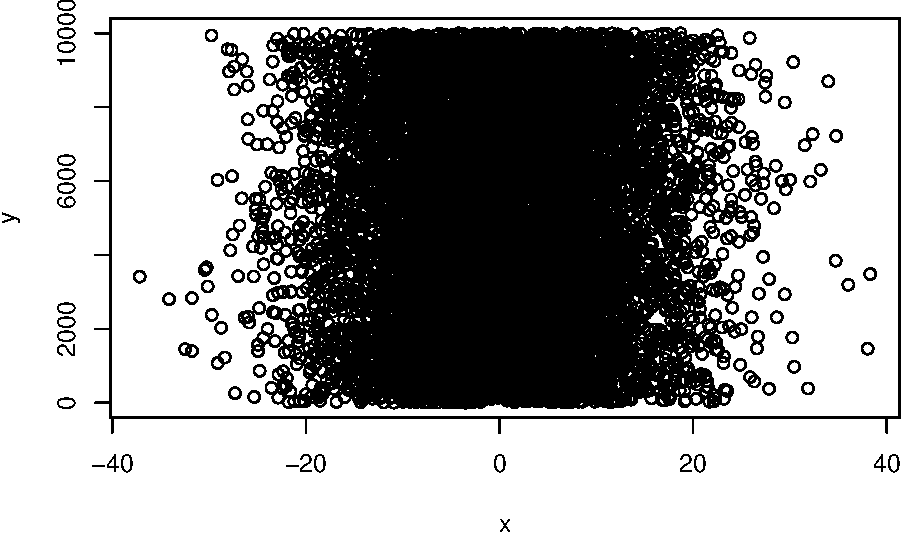
\includegraphics[width=1\linewidth]{foundational_statistics_files/figure-latex/Samples from distributions 1-1}

\begin{itemize}
\item
  You've probably figured out that ``y'' from the last example is a draw of numbers with equal probability (what we call a flat, or uniform distribution).
\item
  What if you want to draw from a distribution?
\item
  Again, play around with the arguments in the parentheses to see what happens.
\end{itemize}

\begin{Shaded}
\begin{Highlighting}[]
\NormalTok{x <-}\KeywordTok{rnorm}\NormalTok{(}\DecValTok{1000}\NormalTok{, }\DecValTok{0}\NormalTok{, }\DecValTok{100}\NormalTok{)}
\KeywordTok{print}\NormalTok{ (x)}
\end{Highlighting}
\end{Shaded}

\begin{verbatim}
##    [1] -9.632411e+01 -2.946647e+00  1.313783e+02 -9.480609e+01 -2.176785e+01
##    [6] -6.902277e+01  1.217067e+02 -4.919045e+01  1.376299e+01  9.325818e+01
##   [11] -1.453173e+02  9.160958e+01  7.042451e+00  5.191549e+01  7.195463e+01
##   [16]  9.965544e+01 -1.166697e+02 -8.964599e+01 -1.825209e+02  1.009805e+02
##   [21]  6.252903e+00  6.076688e+01 -8.660954e+01 -4.090593e+01 -2.008898e+02
##   [26] -7.015944e+01  1.343167e+02  3.362328e+00  5.880706e+01 -3.623925e+01
##   [31]  1.277877e+02 -3.998500e+01 -3.484093e+01 -1.339164e+01 -1.633124e+02
##   [36] -1.635518e+01  3.905313e+01  1.331722e+02 -1.373011e+02 -6.198433e+01
##   [41] -4.875205e+01  9.926274e+01  3.140175e+00  2.969474e+01  2.332572e+01
##   [46] -8.898687e+00  3.499248e+01  4.851585e+01 -1.613946e+02 -1.271991e+02
##   [51]  6.307856e+01  7.909786e+01 -4.924356e+01  1.226313e+01 -2.049451e+01
##   [56]  1.000208e+02 -7.688159e+01 -1.076552e+01  2.097432e+01 -4.074642e+01
##   [61] -6.255335e+01 -8.519156e+01 -2.767848e+01  7.259556e+01  1.213101e+01
##   [66] -6.865817e+01 -1.259162e+02  1.252900e+02  7.250425e+01  1.445048e+02
##   [71]  2.826689e+01  4.428281e+01  6.312902e+01  2.972080e+01 -8.158195e+01
##   [76]  5.928978e+01 -6.077438e+01 -4.215137e+01  1.692347e+00 -8.276484e+01
##   [81] -6.503482e+01  9.030229e+00  1.921182e+02  2.268500e+02  1.752507e+02
##   [86]  1.378213e+02  2.955754e+02  8.780553e+01 -1.215567e+02  1.094922e+02
##   [91]  6.049493e+01  7.788699e+01  5.322968e+01 -1.083615e+02  1.633540e+02
##   [96] -7.300259e+01  1.642928e+02 -3.111706e+01  8.667127e+01 -8.990059e+01
##  [101] -1.511448e+02 -7.787664e+01 -3.640184e+01  5.021656e+01  4.337944e+01
##  [106]  6.831986e+01  1.304706e+02  6.392730e+00  2.865631e+01 -1.923467e+02
##  [111]  5.722541e+01  9.854878e+01 -1.359966e+02  3.550338e+01  4.861449e+01
##  [116]  1.337257e+02  6.623885e+01 -7.164239e+01  2.909886e+01 -4.662361e+01
##  [121]  6.275616e+01  4.681043e+00 -6.119822e+01 -3.495573e+01 -5.706925e+01
##  [126] -1.574845e+02 -2.781019e+01 -3.443886e+01 -3.400346e+01 -1.202975e+02
##  [131] -1.028865e+02  1.345223e+02  2.544974e+01  7.464498e+01 -1.249406e+02
##  [136]  8.614705e+01 -1.929300e+01  1.639148e+02 -7.155742e+01  7.677499e+01
##  [141]  2.972604e+01  5.075692e+01 -7.074975e+01  2.075689e+02  8.712670e+00
##  [146]  5.899291e+00 -2.603035e+01 -1.396319e+01 -1.341926e+01  1.726184e+01
##  [151] -9.072652e+01 -7.822792e+00 -1.783876e+02 -6.951719e+01 -8.329521e+01
##  [156] -1.273539e+02 -2.376056e+02 -1.190907e+02  5.832475e+01 -8.389184e+00
##  [161]  1.201160e+02 -1.868325e+02 -4.288855e+01 -2.550842e+01  8.920134e+01
##  [166] -8.432805e+01  5.098763e+01 -1.035770e+00 -2.221542e+02  1.868706e+02
##  [171] -3.656348e+01 -4.149033e+01  1.459730e+02 -1.193954e+02  2.833110e+02
##  [176] -4.068171e+01 -1.544371e+02 -5.680622e+01  7.764468e+01 -7.256705e+00
##  [181]  4.503894e+01  2.280042e+01  3.040137e+00  7.392931e+01 -1.521450e+02
##  [186] -8.446755e+01  1.175750e+02 -1.067265e+02  1.373877e+02 -1.266127e+02
##  [191]  2.900111e+02  5.143878e+01  2.677810e+01 -1.960169e+02 -1.144241e+00
##  [196] -1.039952e+02  6.479881e+01  1.358096e+02  5.711393e+01  2.199968e+02
##  [201] -8.485430e+01  9.917356e-02 -2.123235e+02  2.524766e+01  6.371120e+01
##  [206]  1.029988e+02  1.000252e+01  1.405151e+01  5.167583e+01 -2.742315e+00
##  [211]  1.449433e+02 -4.239975e+01  7.047416e+01  1.362807e+02 -1.300393e+02
##  [216]  6.587748e+01 -3.079467e+01  3.162797e+01 -1.419183e+01  5.693963e+01
##  [221]  4.363431e+01 -9.270680e+01 -3.820765e+01 -3.084564e+01  3.994561e+01
##  [226]  1.092547e+01 -5.021147e+01  4.047592e+01 -5.836661e+01  4.879898e+01
##  [231]  6.038813e+01  4.560072e+01 -8.660941e+01  9.825662e+01  5.079133e+01
##  [236] -4.759508e+01  7.581111e+01  9.610488e+01 -1.432524e+02  1.371760e+02
##  [241] -3.000739e+01  1.699131e+01 -1.277462e+02 -1.654911e+01 -4.926940e+01
##  [246] -1.813617e+01  5.964411e+01  1.638270e+02 -7.141095e+01 -1.802035e+01
##  [251] -1.067661e+02 -3.565662e+01 -1.162727e+02 -3.538397e+01 -2.702157e+01
##  [256] -3.126035e+02  1.433742e+02 -5.178696e+01  1.148077e+02 -3.131507e+01
##  [261]  8.671968e+01 -1.396525e+02 -1.026743e+02 -4.350522e+01  1.588712e+02
##  [266]  7.857444e+01 -2.402158e+02 -5.374252e+00  1.085156e+02  8.091078e+01
##  [271] -6.249773e+01 -2.468853e+00  1.708820e+00 -1.397036e+02  7.300529e+01
##  [276] -2.877680e+01 -1.798716e+01  2.667128e+01 -9.232577e+01 -2.110803e+01
##  [281]  1.176793e+02 -3.655279e+01  3.884940e+01 -1.657838e+02  5.559963e+01
##  [286] -2.201539e+01  1.362909e+02  3.088568e+01  1.326746e+02 -4.814824e+01
##  [291] -5.635774e+01  1.009186e+02  1.104251e+02 -1.112464e+02 -2.285409e+01
##  [296]  6.331426e+00  7.835113e+00 -2.401437e+02 -1.218013e+02  1.643300e+02
##  [301]  2.704060e+01 -9.266432e+01  5.775971e+01 -7.218742e+01  1.964048e+01
##  [306] -8.789628e+01 -8.240194e-01 -2.058518e+01 -7.520597e+01 -4.098236e+01
##  [311] -5.607751e+01 -1.747447e+01  2.587224e+01 -1.734155e+01 -1.788334e+02
##  [316] -1.491692e+01  4.807637e+01  2.523923e+01 -8.872898e+00  5.691297e+01
##  [321]  1.851195e+02 -1.385800e+02 -1.136834e+02  5.911101e+01 -6.145119e+01
##  [326]  4.107069e+01 -1.138331e+02  8.601329e+01  5.603667e+01 -1.058089e+02
##  [331] -1.802256e+02  1.491332e+02 -1.293818e+02 -1.022609e+02  1.356032e+02
##  [336]  1.512181e+02 -5.894247e+01 -4.883880e+00  6.500841e+01 -2.855792e+01
##  [341]  1.118414e+01 -3.228621e+01 -1.143158e+02 -2.036571e+01  1.154825e+02
##  [346] -6.820513e+01 -6.368369e+01  3.187772e+01  1.395743e+02  5.358236e+01
##  [351]  2.379528e+01  6.651672e+01 -7.712340e-01 -1.224001e+02  1.997318e+02
##  [356] -2.398511e+01  3.906540e+01 -6.499069e+01  3.259685e+01  2.044476e+02
##  [361] -4.449345e+01  1.096166e+02  2.333460e+02  3.934079e+01 -9.076984e+01
##  [366] -8.543076e+01  5.120112e+01  2.906386e+01  5.702113e+01 -4.126197e-01
##  [371] -1.441345e+02  9.395028e-01  1.408054e+01 -8.110283e+01  6.514175e+01
##  [376] -1.463480e+02  1.907694e+02 -6.882346e+01 -2.334587e+00  1.035028e+02
##  [381]  1.090939e+02  2.151777e+01 -6.556306e+00  5.142084e+01 -1.540541e+01
##  [386] -8.684738e+01  1.167559e+02 -2.262589e+02 -2.644830e+02  1.109031e+02
##  [391]  6.977420e+01  9.329498e+01 -8.392115e+01 -1.857329e+01  1.536897e+02
##  [396] -4.479736e+01  1.577224e+02 -1.511114e+02 -1.266306e+02 -1.194619e+02
##  [401]  1.238197e+02 -2.407194e+01 -6.228671e+01 -1.253816e+02  3.405348e-01
##  [406] -1.890644e+02 -3.055084e+02 -2.646561e+01  1.166811e+02 -9.394711e+01
##  [411] -1.327591e+01 -3.565332e+01  1.108846e+02  8.933374e+01  2.174234e+01
##  [416]  1.888519e+02 -8.237874e+01  6.332198e+01 -5.770161e+00  1.178538e+02
##  [421] -5.047875e+01 -8.999629e+01 -4.489108e+01 -3.908257e+01 -1.036047e+02
##  [426]  1.164914e+02  1.194058e+02  1.313459e+02  5.964865e+01  1.221358e+01
##  [431] -7.165196e+01  7.919594e+00 -5.112326e+01 -1.319262e+01 -1.579283e+01
##  [436] -4.400220e+01 -1.524559e+02 -1.825653e+02 -1.323106e+02 -4.915743e+01
##  [441]  2.795146e+01  6.100640e+01  5.870862e+01 -3.342527e+01  2.357855e+01
##  [446] -1.043097e+02  3.024001e+01 -1.927248e+02 -3.634680e+01 -9.433250e+01
##  [451]  1.509546e+02 -1.281711e+02 -1.028420e+02 -1.022912e+02 -9.848921e+01
##  [456]  1.126762e+02 -1.022950e+02  6.254944e+01 -1.341724e+01  5.183440e+01
##  [461]  7.957523e+01  1.367580e+02 -1.553383e+02 -1.930007e+01 -2.406074e+01
##  [466]  2.144203e+01 -1.145699e+02 -1.503301e+02 -8.726628e+01 -1.046818e+02
##  [471]  4.976399e+01  4.027661e+01 -6.823631e+00 -3.886997e-01 -8.605546e+01
##  [476]  1.230212e+02 -3.369318e+01  1.657357e-01 -3.851507e-01 -3.807406e+01
##  [481] -1.195864e+01 -1.921639e+02  1.481283e+02 -3.928103e+01  2.596589e+01
##  [486] -3.617253e+01 -6.141301e+01  1.421086e+02  4.053527e+00  1.920930e+01
##  [491] -2.276686e+02  8.912867e+01 -1.079684e+01 -3.295911e+01 -1.823070e+00
##  [496]  7.415054e+01  6.553642e+01 -3.999012e+01 -5.199661e+01 -1.211854e+01
##  [501] -3.920845e+00  1.053256e+02  1.812013e+00  9.617899e+01 -1.283143e+02
##  [506] -9.507969e+01 -4.219995e+01 -2.374181e+02 -7.777524e+01 -9.009118e+01
##  [511]  1.265222e+02  1.081654e+02  8.211969e+01  8.620803e+01  3.180911e+01
##  [516]  3.419310e+01 -1.454936e+02 -6.388090e+01 -1.487528e+02 -1.143193e+02
##  [521]  1.849124e+02  4.110752e+01 -1.317828e+02 -4.556302e+01  3.882809e+01
##  [526]  2.532924e+01 -1.149329e+02  2.583072e+01 -8.254706e+01  5.733686e+01
##  [531] -7.569305e+01  9.865659e+01 -4.674082e+01  8.572595e+01  1.588345e+02
##  [536]  1.365000e+01  2.896219e+01  5.597367e+01  9.537225e+01 -8.631454e+01
##  [541]  7.321559e+01 -1.859776e+01 -8.567348e+01  1.320364e+02 -7.336111e+01
##  [546] -1.662205e+01 -4.925110e+01 -1.072929e+02 -5.778051e+01  7.880813e+00
##  [551] -3.001144e+01  6.102117e+01 -1.914918e+00  5.608385e+01 -4.243316e+00
##  [556] -2.293509e+01  8.939485e+01  1.102060e+02 -1.580026e+02  1.057391e+02
##  [561]  2.026081e+01 -2.650916e+01 -1.829339e+02 -1.496983e+01  7.059417e+01
##  [566] -1.065498e+02  1.250187e+02  6.951958e+01  3.869608e+01  8.371719e+01
##  [571] -8.150094e+01  1.091408e+02 -7.264239e+01 -4.183778e+01 -1.978531e+01
##  [576] -2.481549e+01  1.889573e+01  1.037666e+02  1.375203e+02 -3.570707e+01
##  [581] -6.486770e+01 -4.379172e+01  8.853807e+01  1.063544e+01 -3.920313e+01
##  [586]  1.593278e+02 -1.755889e+02  4.256121e+01 -8.223893e+01  3.895314e+00
##  [591] -9.509101e+01 -1.637086e+02  1.337099e+02 -8.685364e+01  9.995676e+00
##  [596]  1.965327e+02 -1.366256e+02 -3.148484e+01  9.548940e+01  1.562852e+02
##  [601] -1.201817e+02  4.360627e+00  3.900634e+01 -2.329831e+02 -5.932206e+01
##  [606] -9.672414e+01  3.505079e+01 -6.721509e+00 -1.965768e+02  1.478660e+02
##  [611] -1.542613e+02  7.236708e+01  1.107052e+02  8.747391e+01  9.529106e+01
##  [616]  3.582387e+01  8.308489e+01 -8.668761e+00  9.598227e+01 -8.596283e+01
##  [621]  1.200841e+01 -5.772102e+01 -6.264569e+01 -1.859903e+01  2.014001e+02
##  [626] -7.427240e+01 -2.265722e+01 -2.437090e+01 -2.133346e+01  6.642049e+01
##  [631] -1.421570e+01 -3.033463e+01 -9.978815e+01 -4.827290e+01 -2.227630e+00
##  [636] -9.813082e+00  2.216067e+01  1.369490e+02 -1.365663e+02  7.354403e+01
##  [641]  3.522018e+01 -3.277792e+01 -2.263976e+01 -3.701086e+01 -1.987911e+02
##  [646]  2.451724e+01 -6.338506e+01  1.058587e+02  2.678512e+02  1.339453e+02
##  [651] -6.242527e+01 -8.958057e+01 -7.995812e+01  3.016585e+01 -1.739943e+02
##  [656]  3.436805e+01  3.757583e+01 -4.994822e+01  1.847981e+02 -7.287585e+01
##  [661]  4.030974e+01 -9.147180e+01  1.229114e+02  2.712884e+01 -3.811247e+01
##  [666]  9.550231e+01  2.261274e+02 -9.087736e+01  1.340559e+02  7.540179e+01
##  [671] -1.281451e+01 -7.322630e+01 -1.224938e+01 -1.729696e+02  1.902332e+02
##  [676]  1.021067e+02  9.845653e+01  4.605987e+01  1.741151e+02  7.065228e+01
##  [681]  6.328805e+01  8.788754e+01  1.443435e+02  7.714077e+01  1.965453e+02
##  [686]  3.503461e+01 -1.530337e+01 -6.935420e+01 -2.740559e+00  2.281459e+01
##  [691]  2.675274e+01 -9.355365e+01 -1.124817e+01  1.167142e+01 -1.328469e+02
##  [696] -1.729077e+01  9.490001e+01 -2.041649e+01  8.108525e+01 -1.025042e+02
##  [701] -6.479063e+01  4.838856e+00  1.345383e+02  8.195719e+01  2.742820e+02
##  [706]  7.528146e+01 -7.201496e+01  5.739326e+01  1.340256e+02  4.508085e-03
##  [711] -6.614753e+01 -4.985802e+01  1.016060e+02  2.998868e+01  1.055259e+02
##  [716] -1.964175e+02 -2.624484e+01  1.925031e+02  1.587370e+02 -4.760702e+01
##  [721]  8.556741e+01  5.702033e+01 -5.863248e+01  8.066524e+01 -4.575569e+01
##  [726] -6.405493e+01  8.923198e+01 -4.117726e+01 -1.303796e+02  1.947045e+01
##  [731] -5.776675e+01  4.159134e+01  1.004072e+01  6.715970e+01  7.794020e+01
##  [736] -5.962927e+01  7.078611e+01 -7.225475e+01 -1.553864e+02  3.901645e+01
##  [741] -7.391585e+01  1.611866e+02 -5.694669e+01 -2.085814e+02 -1.539142e+02
##  [746] -7.427986e+01 -4.258104e+01 -2.431742e+01 -7.755738e+01 -2.567634e+01
##  [751] -1.123901e+02  7.215657e+01 -2.533908e+01 -1.263971e+02 -2.156903e+01
##  [756]  1.503232e+02  1.323775e+02 -1.381415e+02 -8.509368e+01 -7.748420e+00
##  [761]  9.395214e+01  6.971698e+01 -3.025405e+01  1.190802e+02 -4.675354e+01
##  [766] -4.291207e+00  4.928402e+01  3.986277e+00 -2.420144e+01 -2.622542e+01
##  [771] -9.121144e+01 -6.634909e+01 -3.065351e+01 -1.113056e+02  9.774857e-01
##  [776] -8.653542e+01  1.531898e+01 -1.484764e+02  1.027073e+02  1.191334e+02
##  [781]  8.079541e+01 -1.326184e+02  7.668478e+01  6.998787e+01  2.225859e+02
##  [786] -9.746936e+01 -1.631121e+02 -3.384048e+01  3.302569e+01  3.687808e+01
##  [791] -8.189613e+01 -6.747353e+01  9.938360e+01  1.219446e+02 -1.049275e+02
##  [796] -2.894126e+01 -8.661852e+00  1.191198e+02 -8.857771e+01  1.836779e+02
##  [801] -8.514820e+01 -5.820340e+01  8.171538e+01  9.733134e+01 -6.801310e+01
##  [806]  1.759763e+00 -1.106434e+02 -1.455405e+00 -1.854861e+02 -1.070496e+02
##  [811]  1.646613e+02 -6.339518e+01 -1.262067e+02 -1.490989e+02  9.406135e+01
##  [816] -1.930688e+01 -4.036816e+01 -3.417009e+01 -8.580004e+01  1.197862e+02
##  [821] -1.801420e+02 -6.249816e+01 -9.611559e+01  1.661881e+02 -1.575072e+02
##  [826]  1.316233e+02  3.045032e+01  4.875284e+01  7.692344e+01 -3.109959e+01
##  [831] -1.222723e+02 -5.053869e+01 -7.277502e+01 -2.771258e+01  1.722247e+02
##  [836] -9.015410e+01 -1.365412e+02 -8.494124e+01 -1.097742e+02  3.563410e+01
##  [841]  5.687477e+01 -1.425916e+01 -7.929238e+00 -2.478807e+02  7.832968e+01
##  [846] -1.007460e+02 -1.173860e+02  2.129740e+01  2.622033e+02  5.660083e+01
##  [851]  9.734236e+01 -3.434605e+01  9.716732e+00 -1.012788e+01  9.939509e+01
##  [856] -6.936073e+01  1.386178e+02  3.874617e+01  3.219052e+01 -2.586483e+01
##  [861]  6.167873e+01 -4.273083e+01  5.151848e+01 -9.842675e+01 -2.498785e+01
##  [866] -1.135727e+02 -1.740705e+02  1.159547e+02  2.186337e+00  1.695844e+02
##  [871]  1.471802e+02 -1.349718e+02 -7.585076e+01 -1.016018e+02 -7.079777e+01
##  [876] -1.166189e+02  2.502812e+01  5.220238e+01 -3.765801e+01 -6.029564e+01
##  [881]  1.388687e+00  1.306913e+02 -1.178755e+02  1.833873e+01 -1.396343e+02
##  [886]  2.257843e+00  7.901024e+01 -4.260354e+00  1.444804e+02 -5.998962e+01
##  [891] -3.326110e+01 -1.625563e+02 -1.257131e+02  7.666526e+01  9.918874e+01
##  [896]  5.534856e+01 -7.137956e+01  3.415869e+01  4.168533e+00 -2.437278e+01
##  [901] -3.745845e+01 -1.075850e+02  2.536468e+02  8.959670e+01  9.292464e+01
##  [906] -1.866057e+02  1.205549e+02  1.203846e+01 -2.748793e+01  1.573858e+02
##  [911]  1.120433e+02 -2.408124e+02  1.611804e+01  6.776519e+01  4.931427e+01
##  [916] -7.282368e+00 -9.570613e+01 -5.458058e+01  2.137207e+02  3.867011e+01
##  [921] -5.148826e+01 -1.576149e+02  8.060121e+01 -1.934120e+01 -6.224347e+01
##  [926]  5.750517e+00  7.861141e+01  1.334782e+02  1.615862e+02 -6.437721e+01
##  [931] -4.281610e+01 -3.559026e+01 -2.219572e+01 -7.622408e+01 -9.991926e+01
##  [936] -1.052987e+02  4.106839e+01 -1.288628e+02 -9.637850e+01 -2.104430e+01
##  [941]  4.629157e+01  1.917738e+01 -7.489351e+01 -1.815277e+00  1.915721e+02
##  [946] -3.568372e+01 -4.753921e+01  4.865418e+01 -7.062431e+01  4.942442e+01
##  [951] -3.754630e+01  1.712584e+01 -1.771198e+01 -3.007542e+01 -1.662739e+02
##  [956]  5.078226e+00  5.402923e+01 -1.687089e+02 -2.124013e+01 -5.564933e+01
##  [961] -5.521287e+01  6.748005e-01  4.617274e+01  3.160277e+01  2.677520e+01
##  [966]  2.710642e+01 -6.344277e+01 -9.797320e+01 -1.649687e+02 -2.586085e+01
##  [971] -6.728047e+01 -1.414794e+02  1.018355e+02  2.838364e+01 -1.327246e+02
##  [976] -8.257584e+01 -6.530273e+01  9.052841e+01 -1.553269e+02  3.088988e+01
##  [981] -1.865751e+02 -6.305439e+01 -6.259455e+01 -7.185359e+01  4.949858e+01
##  [986]  1.065410e+02  7.641417e+01 -5.075361e+01  1.991034e+00 -1.153476e+02
##  [991] -2.552500e+02  2.663271e+01  3.393291e+00 -1.866147e+02  6.882899e+01
##  [996]  4.943874e+01 -4.533336e+01  9.554360e+00  1.849825e+01  2.044823e+02
\end{verbatim}

\begin{Shaded}
\begin{Highlighting}[]
\KeywordTok{hist}\NormalTok{(x, }\DataTypeTok{xlim =} \KeywordTok{c}\NormalTok{(}\OperatorTok{-}\DecValTok{50}\NormalTok{,}\DecValTok{50}\NormalTok{))}
\end{Highlighting}
\end{Shaded}

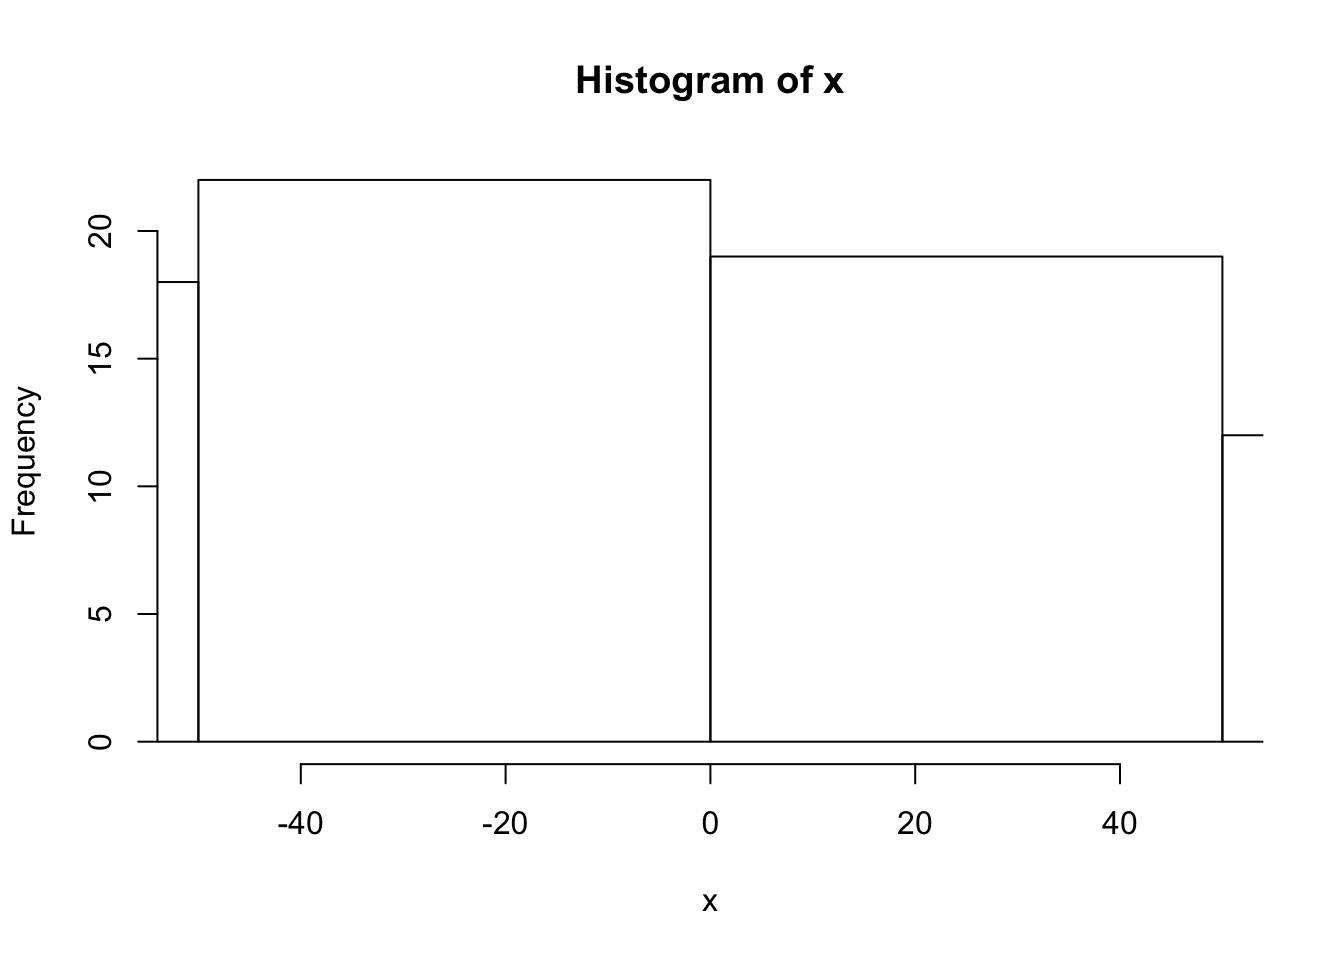
\includegraphics[width=1\linewidth]{foundational_statistics_files/figure-latex/Samples from distributions 2-1}

\begin{Shaded}
\begin{Highlighting}[]
\KeywordTok{hist}\NormalTok{(x, }\DataTypeTok{xlim =} \KeywordTok{c}\NormalTok{(}\OperatorTok{-}\DecValTok{500}\NormalTok{,}\DecValTok{500}\NormalTok{))}
\end{Highlighting}
\end{Shaded}

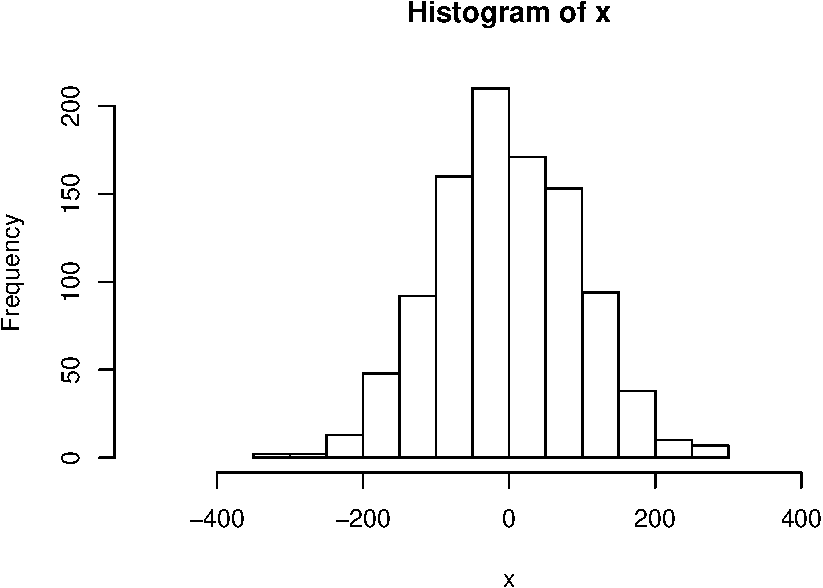
\includegraphics[width=1\linewidth]{foundational_statistics_files/figure-latex/Samples from distributions 2-2}

Can you figure out what the three rnorm() arguments represent?

\hypertarget{basic-summary-statistics}{%
\subsubsection{Basic Summary Statistics}\label{basic-summary-statistics}}

We will get into the details regarding summary statistics later, but for now, check out several of the \texttt{R} functions that calculate them.

\begin{Shaded}
\begin{Highlighting}[]
\KeywordTok{mean}\NormalTok{(x)}
\KeywordTok{median}\NormalTok{(x)}
\KeywordTok{var}\NormalTok{(x)}
\KeywordTok{log}\NormalTok{(x)}
\KeywordTok{ln}\NormalTok{(x)}
\KeywordTok{sqrt}\NormalTok{(x)}
\KeywordTok{sum}\NormalTok{(x)}
\KeywordTok{length}\NormalTok{(x)}
\KeywordTok{sample}\NormalTok{(x, }\DataTypeTok{replace =}\NormalTok{ T)}
\end{Highlighting}
\end{Shaded}

\begin{itemize}
\item
  Notice that the last function (\texttt{sample}) has an argument (\texttt{replace=T})
\item
  Arguments simply modify or direct the function in some way
\item
  There are many arguments for each function, some of which are defaults
\end{itemize}

\hypertarget{getting-help-to-understand-functions}{%
\subsubsection{Getting help to understand functions}\label{getting-help-to-understand-functions}}

\begin{itemize}
\item
  Getting help on any function is very easy - just type a question mark and the name of the function.
\item
  There are functions for just about anything within \texttt{R} and it is easy enough to write your own functions if none already exist to do what you want to do.
\item
  In general, function calls have a simple structure: a function name, a set of parentheses and an optional set of arguments you assign parameters to and send to the function.
\item
  Help pages exist for all functions that, at a minimum, explain what parameters exist for the function.
\item
  Help can be accessed a few ways - try them :
\end{itemize}

\begin{Shaded}
\begin{Highlighting}[]
\OperatorTok{-}\StringTok{ }\KeywordTok{help}\NormalTok{(mean)}
\OperatorTok{-}\StringTok{ }\NormalTok{?mean}
\OperatorTok{-}\StringTok{ }\KeywordTok{example}\NormalTok{(mean)}
\OperatorTok{-}\StringTok{ }\KeywordTok{help.search}\NormalTok{(}\StringTok{"mean"}\NormalTok{)}
\OperatorTok{-}\StringTok{ }\KeywordTok{apropos}\NormalTok{(}\StringTok{"mean"}\NormalTok{)}
\OperatorTok{-}\StringTok{ }\KeywordTok{args}\NormalTok{(mean)}
\end{Highlighting}
\end{Shaded}

\hypertarget{exercises-associated-with-this-chapter-1}{%
\section{Exercises associated with this chapter:}\label{exercises-associated-with-this-chapter-1}}

\begin{itemize}
\tightlist
\item
  Exercise 2 (file: \texttt{rtutorial\_1.Rmd})
\end{itemize}

\hypertarget{additional-learning-resources-1}{%
\section{Additional learning resources:}\label{additional-learning-resources-1}}

\begin{itemize}
\item
  Logan, M. 2010. Biostatistical Design and Analysis Using R. - A great intro to R for statistical analysis
\item
  \url{http://library.open.oregonstate.edu/computationalbiology/} - O'Neil, S.T. 2017. A Primer for Computational Biology
\end{itemize}

\bibliography{book.bib,packages.bib}

\end{document}
